\documentclass[11pt,letterpaper]{article}
\input{headings}
\newcommand \recipeName {Pigs in a Blanket}
\newcommand \fileName {PigsOnBlanket}
\chead{\recipeName}

\begin{document}
\input{title}

For the dough, I use the recipe for the ``Best American Dinner Rolls" from {\it Cook's Illustrated}. For a dairy-free version replace the milk for almond milk and the butter for baking margarine. This recipe is very convenient for a party or celebration, because the dough is prepared and the pigs in a blanket are formed up to two days before baking and serving. They must be removed from the refrigerator and put to rise in a cool room temperature 6 to 7 hours before baking.

\vspace{0.3in}
\begin{description}

\item[Ingredients:]\ \\
	\begin{itemize}
	\item 3/4 cup whole milk (6 1/4 oz)
	\item 6 tablespoons unsalted butter, melted (3 oz) 
	\item 6 tablespoons sugar (3 oz)
	\item 1 1/2 teaspoons table salt
	\item 2 large eggs , room temperature
	\item 1 package rapid-rise yeast (2 1/4 teaspoons), may also labeled "instant" (8 grams)
	\item 3 cups unbleached all-purpose flour (15 oz)
	\item hot dogs (10 jumbo or 700 grams)
	\item 2 tablespoons unsalted butter , melted (for brushing the pigs before baking) (1 oz)
	\end{itemize}

\item[Procedure:]\ \\
	\begin{enumerate}
	\item {\bf Make the dough base}
		\begin{itemize}
		\item Bring milk to boil in small saucepan over medium heat; let stand off heat until skin forms on surface,
3 to 5 minutes. Using soup spoon, skim skin off surface and discard. 
		\item Transfer milk to bowl of standing mixer and add 6
tablespoons melted butter, sugar, and salt. 
		\item Whisk to combine and let mixture cool. 
		\item When mixture is just warm to the touch (90 to 100 F degrees), whisk in eggs and yeast until combined.
		\end{itemize}

	\item {\bf Add the flour}
		\begin{itemize}
		\item Add flour to  the bowl; using dough hook, mix on low speed on standing mixer until combined, 1 to 2 minutes. 
		\item Increase speed to medium-low and knead about 3 minutes more; when pressed with finger, dough should feel tacky and moist but should not stick
to finger. (If dough is sticky, add another 1 to 3 tablespoons flour.) 
		\item Continue to knead on medium-low until cohesive, elastic dough
has formed (it should clear sides of bowl but stick to bottom), 4 to 5 minutes longer.
		\end{itemize}
		
	\item {\bf Knead the dough}
		\begin{itemize}
		\item Transfer dough to lightly floured work surface. 
		\item Knead dough by hand 1 to 2 minutes to ensure that it is well kneaded. Dough
should be very soft and moist but not overly sticky. (If dough sticks excessively to hands and work surface, knead in flour a
tablespoon at a time until dough is workable.) 
		\item Lightly spray medium bowl with nonstick cooking spray. 
		\item Transfer dough to bowl.
		\item Lightly coat surface of dough with cooking spray and cover with plastic wrap. 
		\item Let dough rise in warm, draft-free location until doubled in volume, 2 to 3 hours.
		\end{itemize}
		
	\item {\bf Prepare baking sheets}
		\begin{itemize}
		\item Spray two baking sheets with cooking spray.
		\item Put two tablespoon of flour in a small strainer and use it to dust the baking sheet. Then bang the baking sheet on the counter several times until it is evenly coated with the flour.
		\item Pour any excessive flour into the sink. 
		\end{itemize}

	\item {\bf Shape the pigs}
		\begin{itemize}
		\item Roll the dough into a 18 in x 24 in rectangular shape. Trim the edges to make them straight.
		\item Cut hot dogs into thirds. Jumbo hot dogs are 6 1/2 in long. Thus each third will measure 2 1/8 in.
		\item Using a piece of hot dog as a guide, make several small slits to mark a strip of dough that is wide enough to roll the hot-dog pieces with enough left in the ends to enclose complitely.
		\item Using the slits as guide cut the strips. 
		\item Roll each hot dog cutting the dough strip to make a closed seam. 
		\item Press along the seam and place seam-side down on the prepared trays.
		\end{itemize}
		
	\item {\bf Refrigerate for a day or two}
		\begin{itemize}
		\item Cover the baking sheets with plastic wrap lightly coated with cooking spray.
		\item Cover the pans securely with foil. 
		\item Refrigerate at least 24 or up to 48 hours.
		\end{itemize}

	\item {\bf Let the pigs raise}
		\begin{itemize}
		\item Remove foil (but not plastic wrap) from baking pans.
		\item Let pigs rise in draft-free cool room-temperature
location until doubled in volume, 6 to 7 hours. 
		\item When pigs are nearly doubled in volume,
adjust oven rack to lower-middle position and heat oven to 400 F.
		\end{itemize}

	\item {\bf Bake the pigs}
		\begin{itemize}
		\item Remove plastic wrap. 
		\item Brush the pigs with 2 tablespoons of melted butter; 
		\item Bake until deep golden brown, 14 to 18 minutes. Rotate pans halfway through to ensure even baking.  
		\item Slightly cool pigs in the pans on wire rack about 3 minutes.
		\item Move the pigs to a rack and cool for 10 to 15 minutes longer. 
		\item Serve warm.
		\end{itemize}
	\end{enumerate}
\end{description}

\begin{table}
\begin{tabular}{cccc}
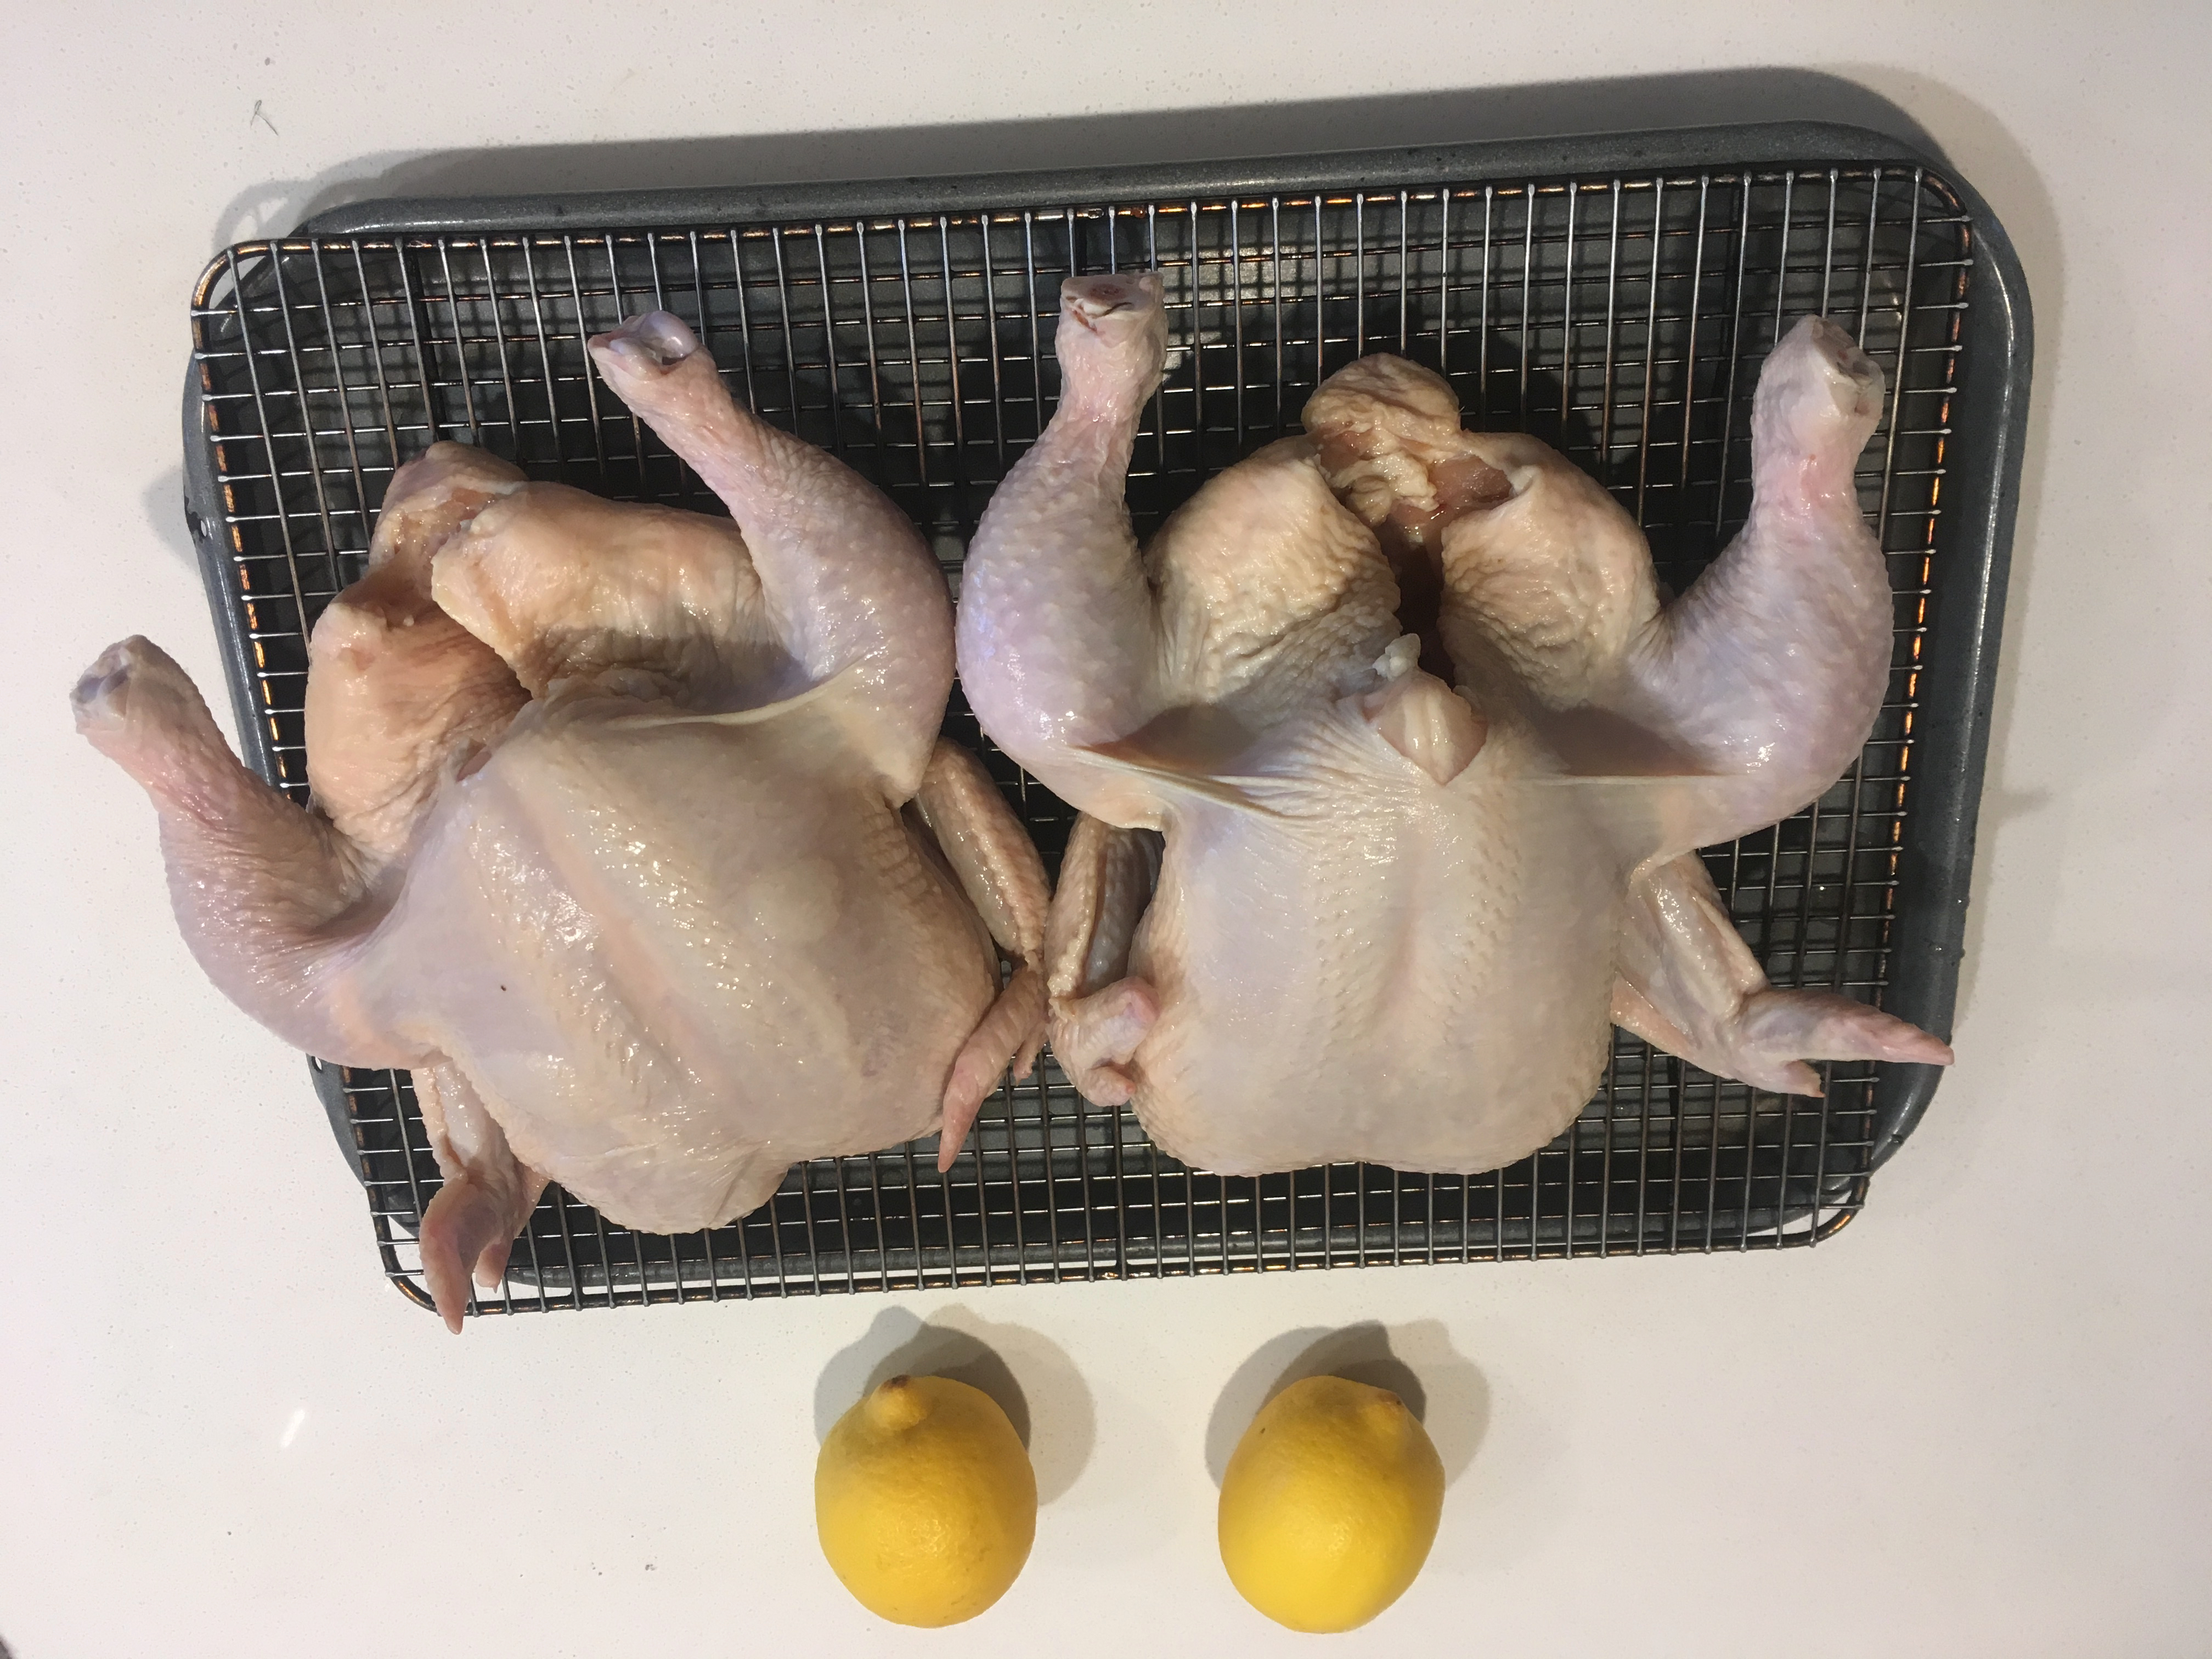
\includegraphics[width=0.25\textwidth]{\imageDir/\fileName/IMG_3197.jpg} &
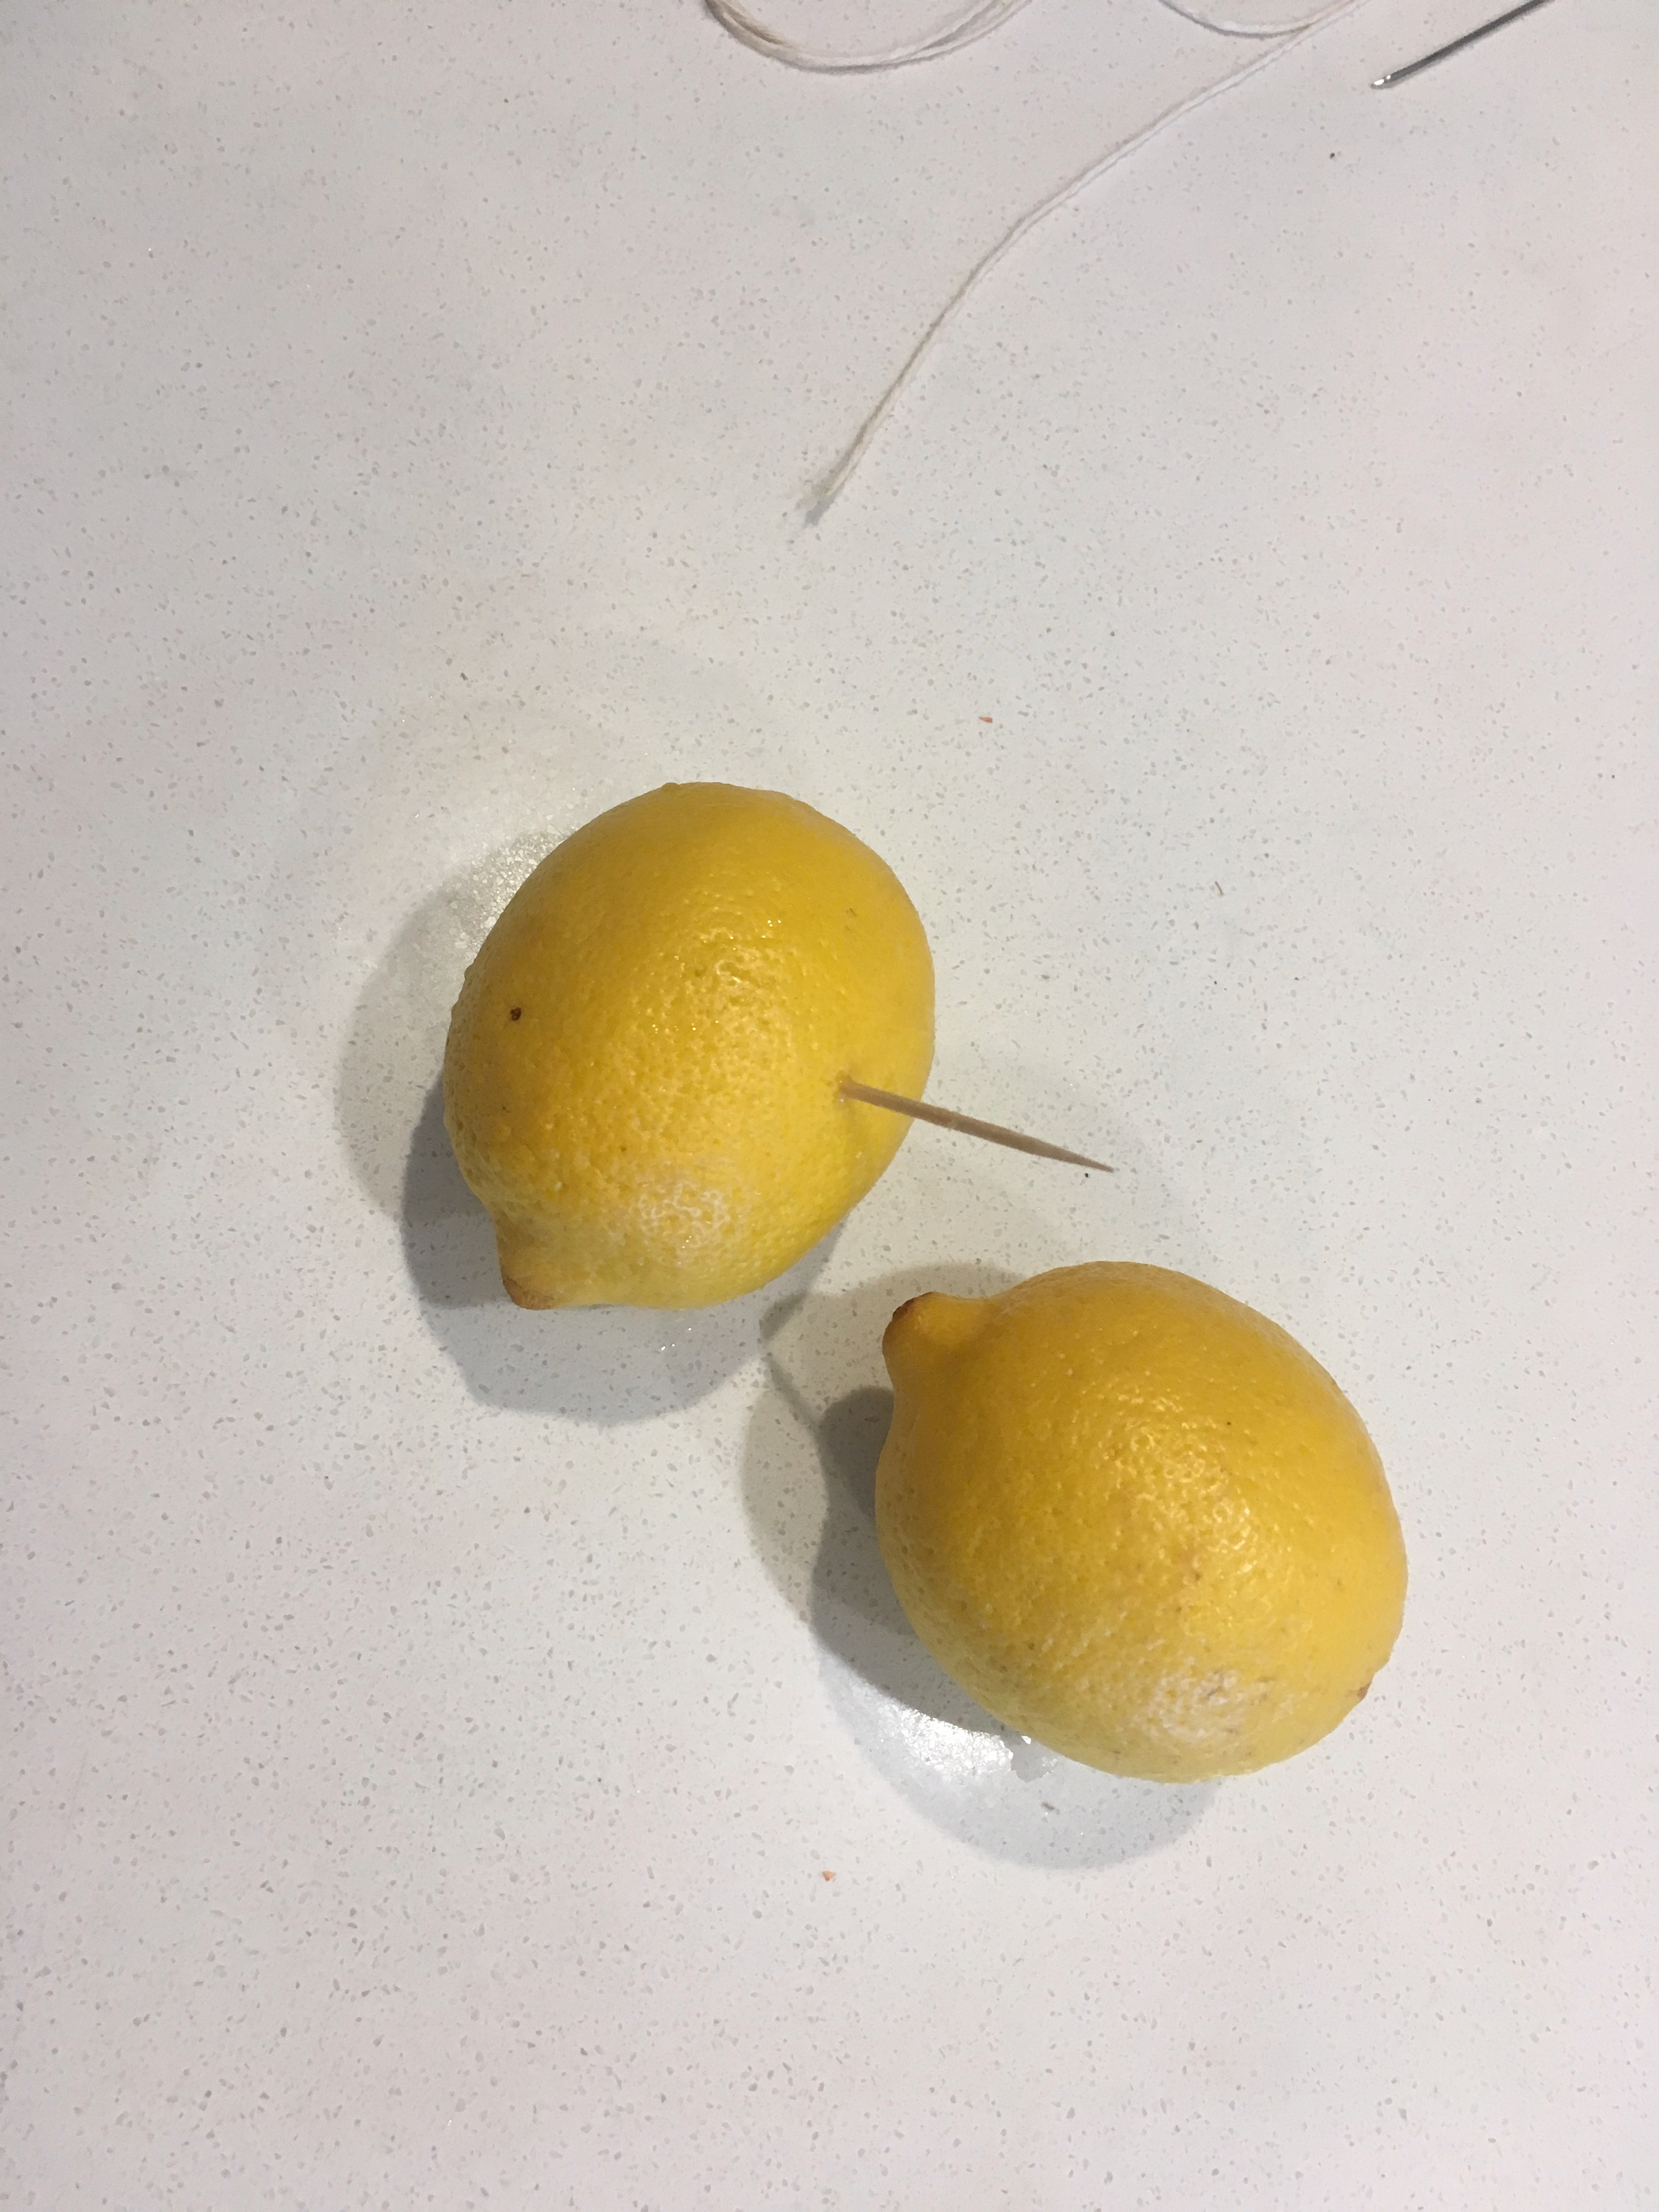
\includegraphics[width=0.25\textwidth]{\imageDir/\fileName/IMG_3212.jpg} &
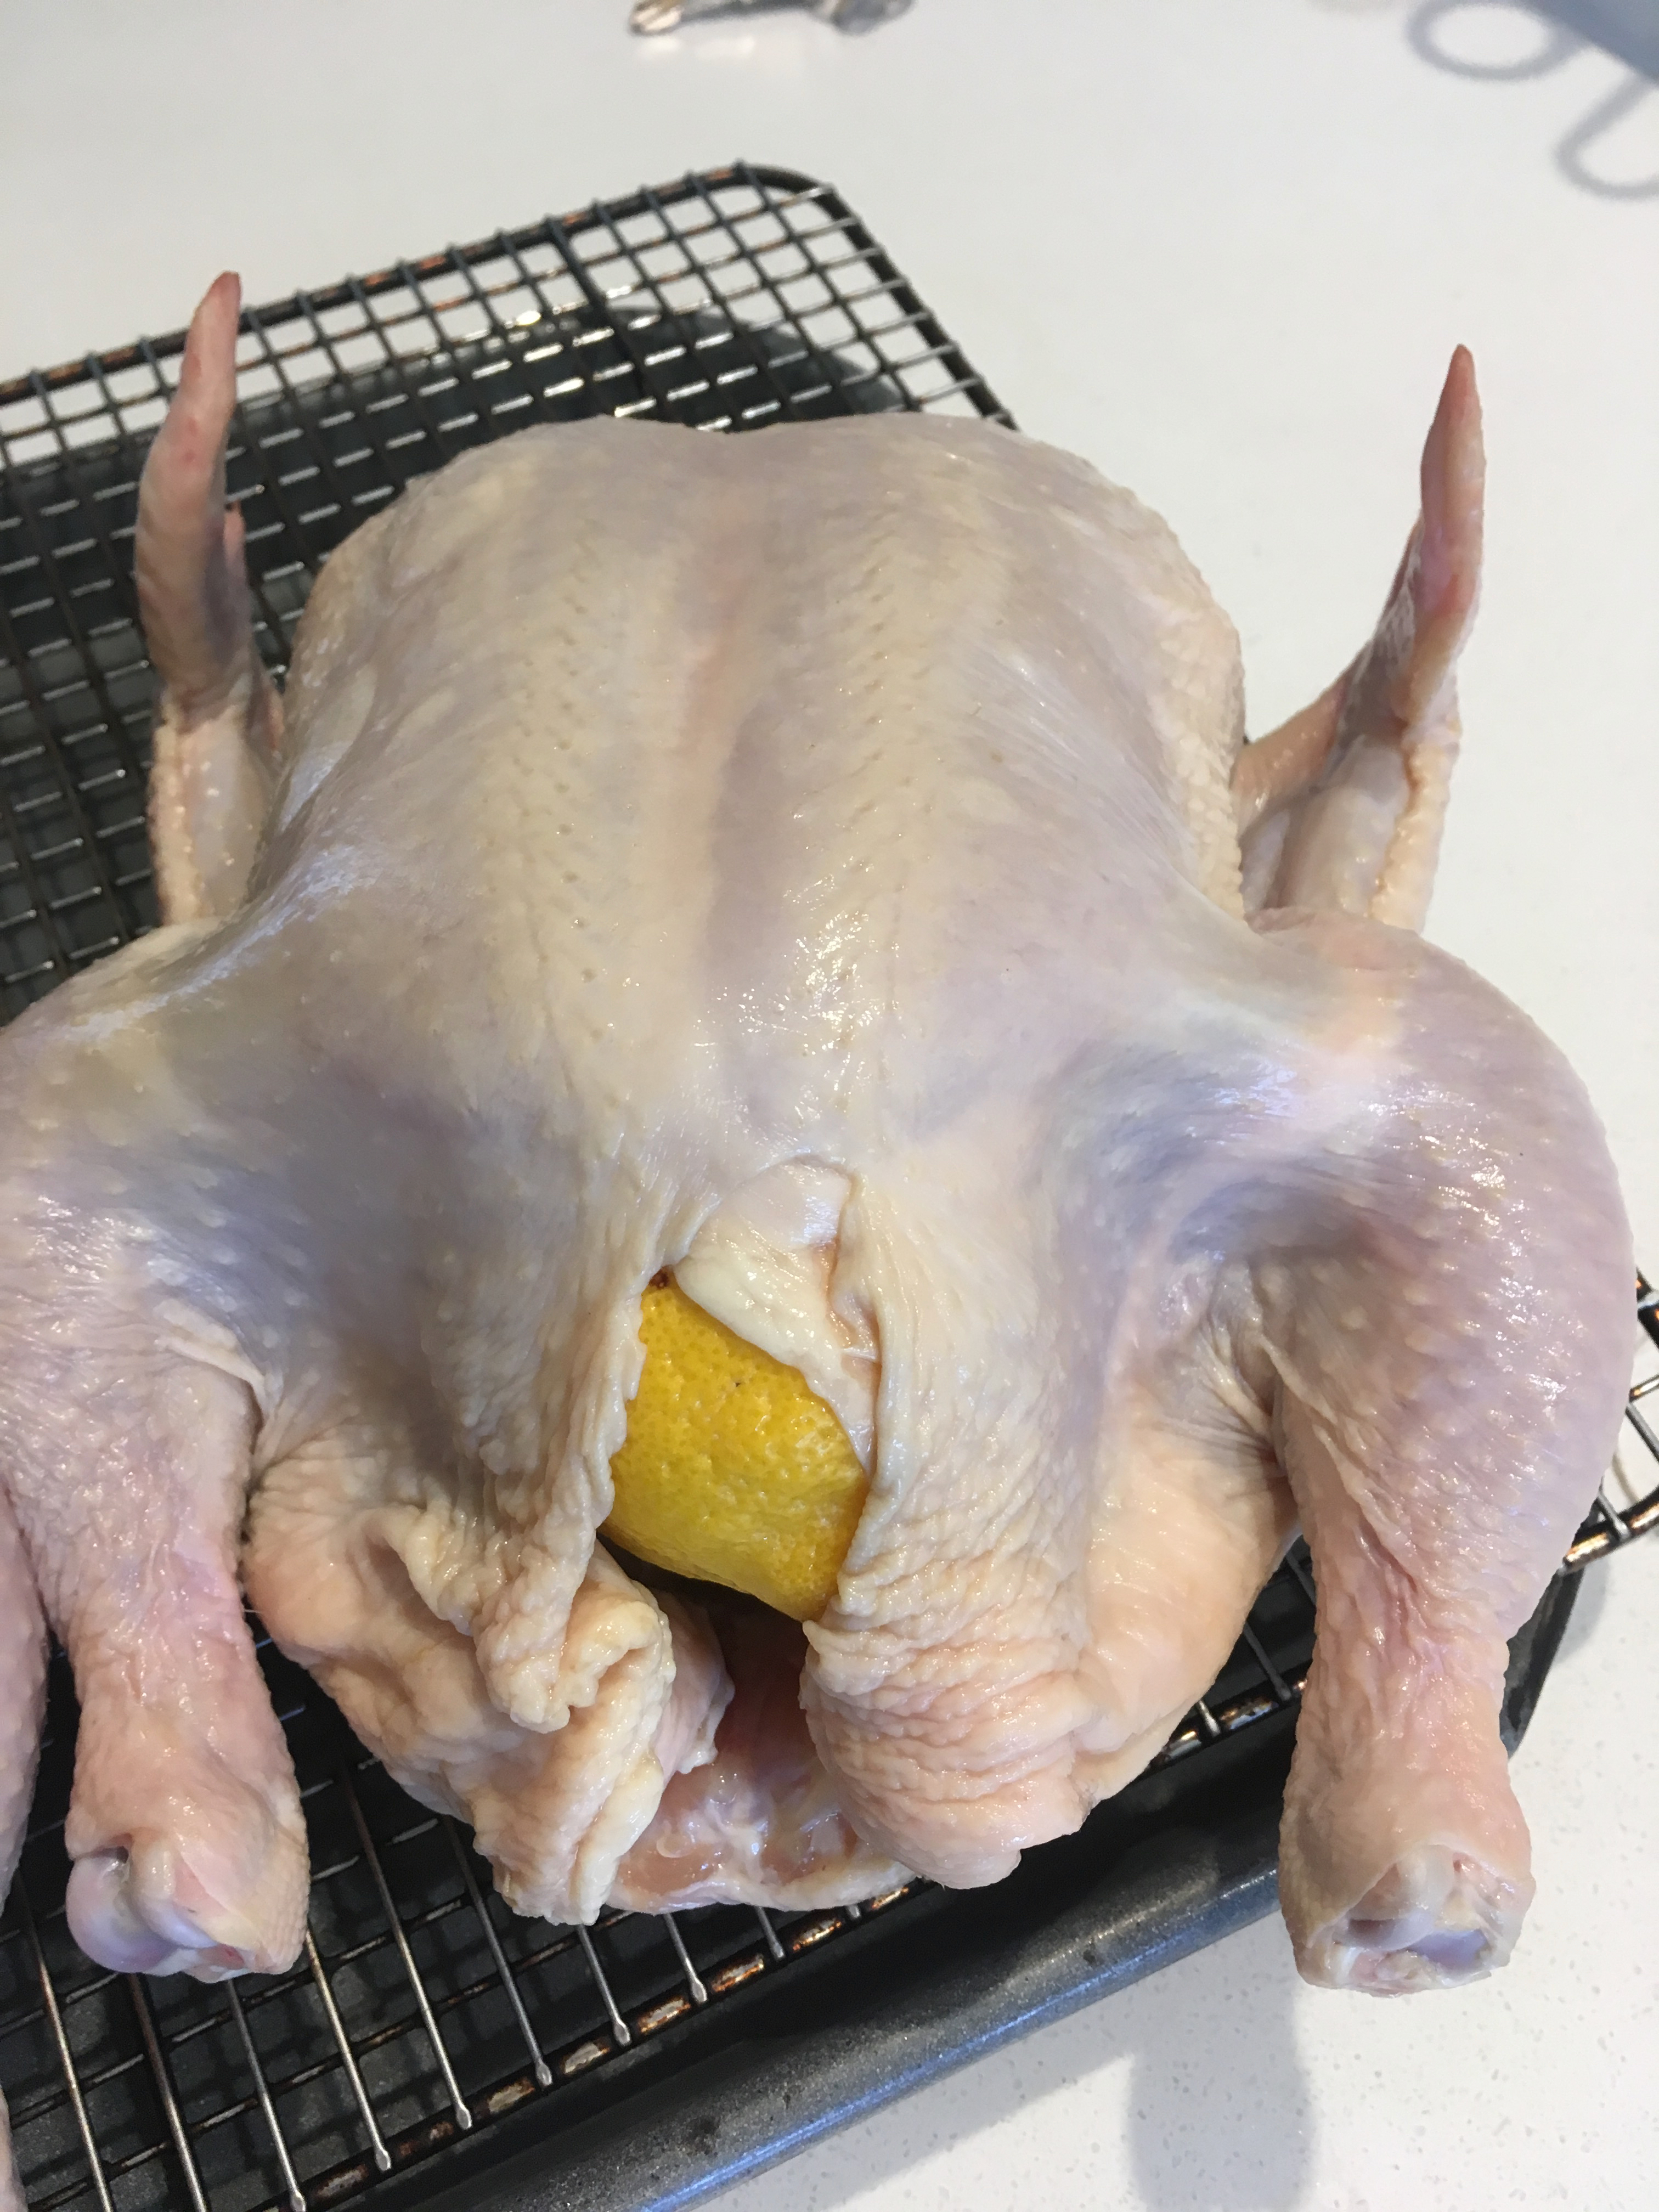
\includegraphics[width=0.25\textwidth]{\imageDir/\fileName/IMG_3213.jpg} \\
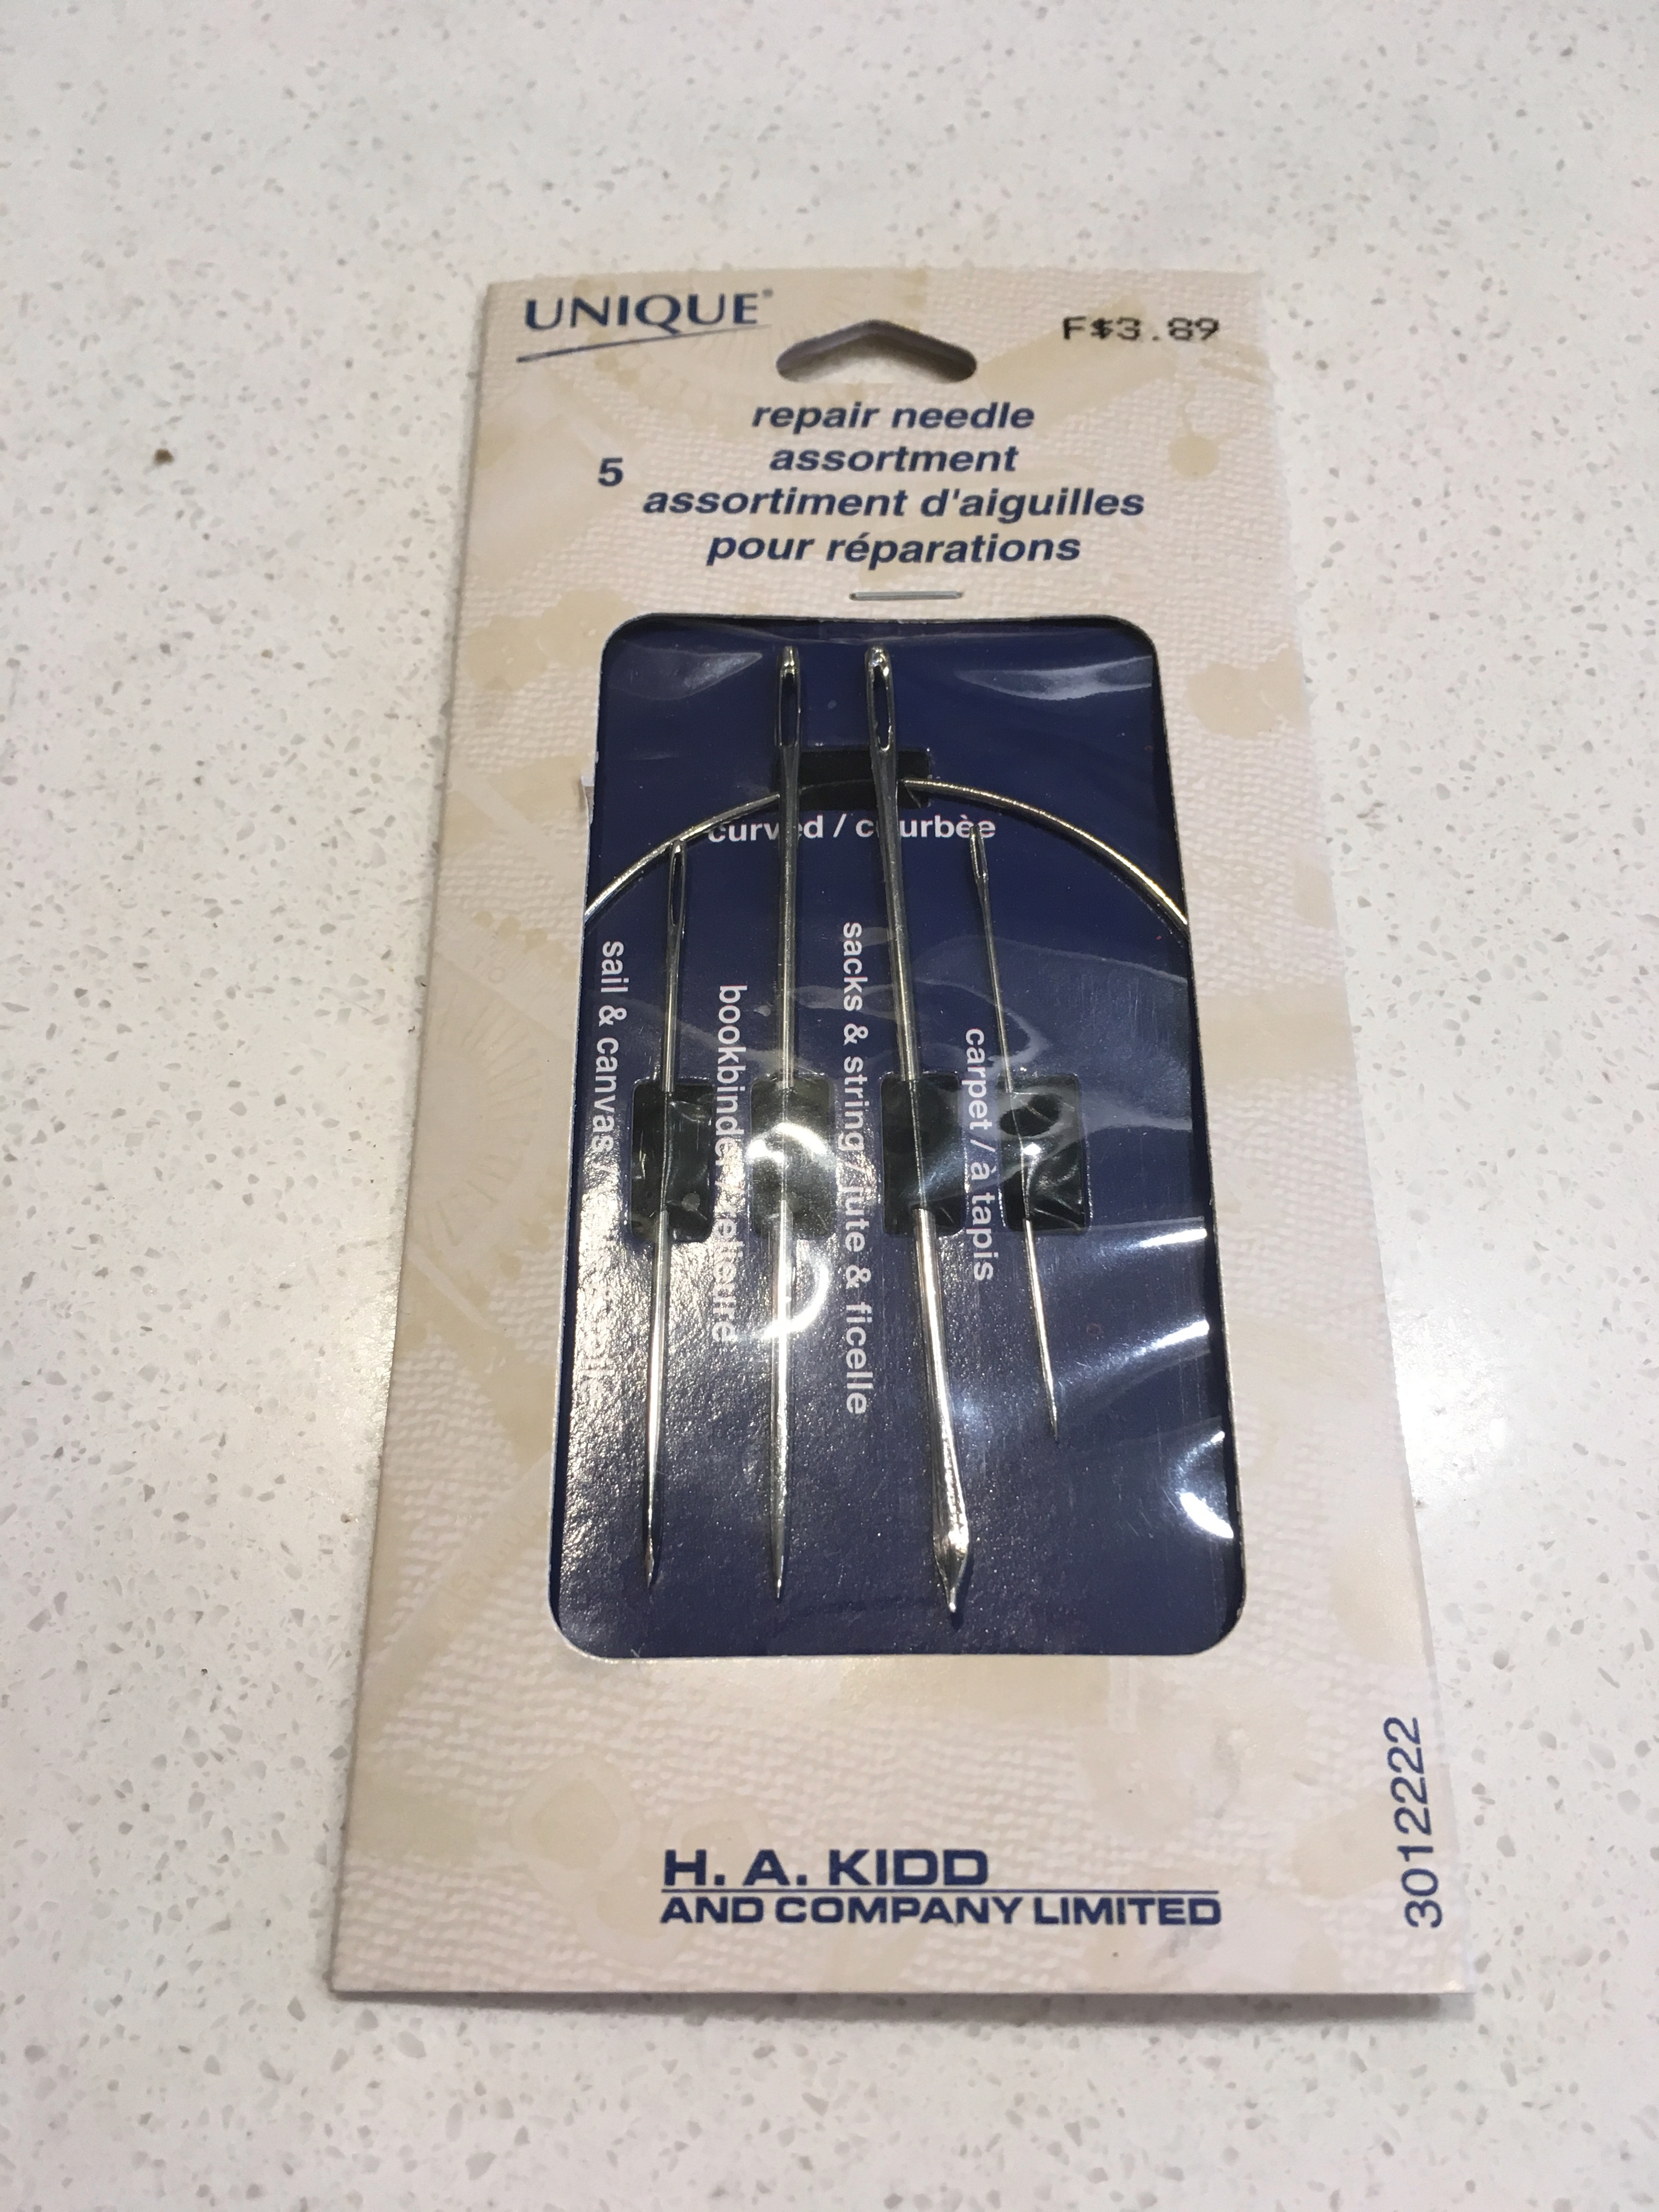
\includegraphics[width=0.25\textwidth]{\imageDir/\fileName/IMG_3206.jpg} &
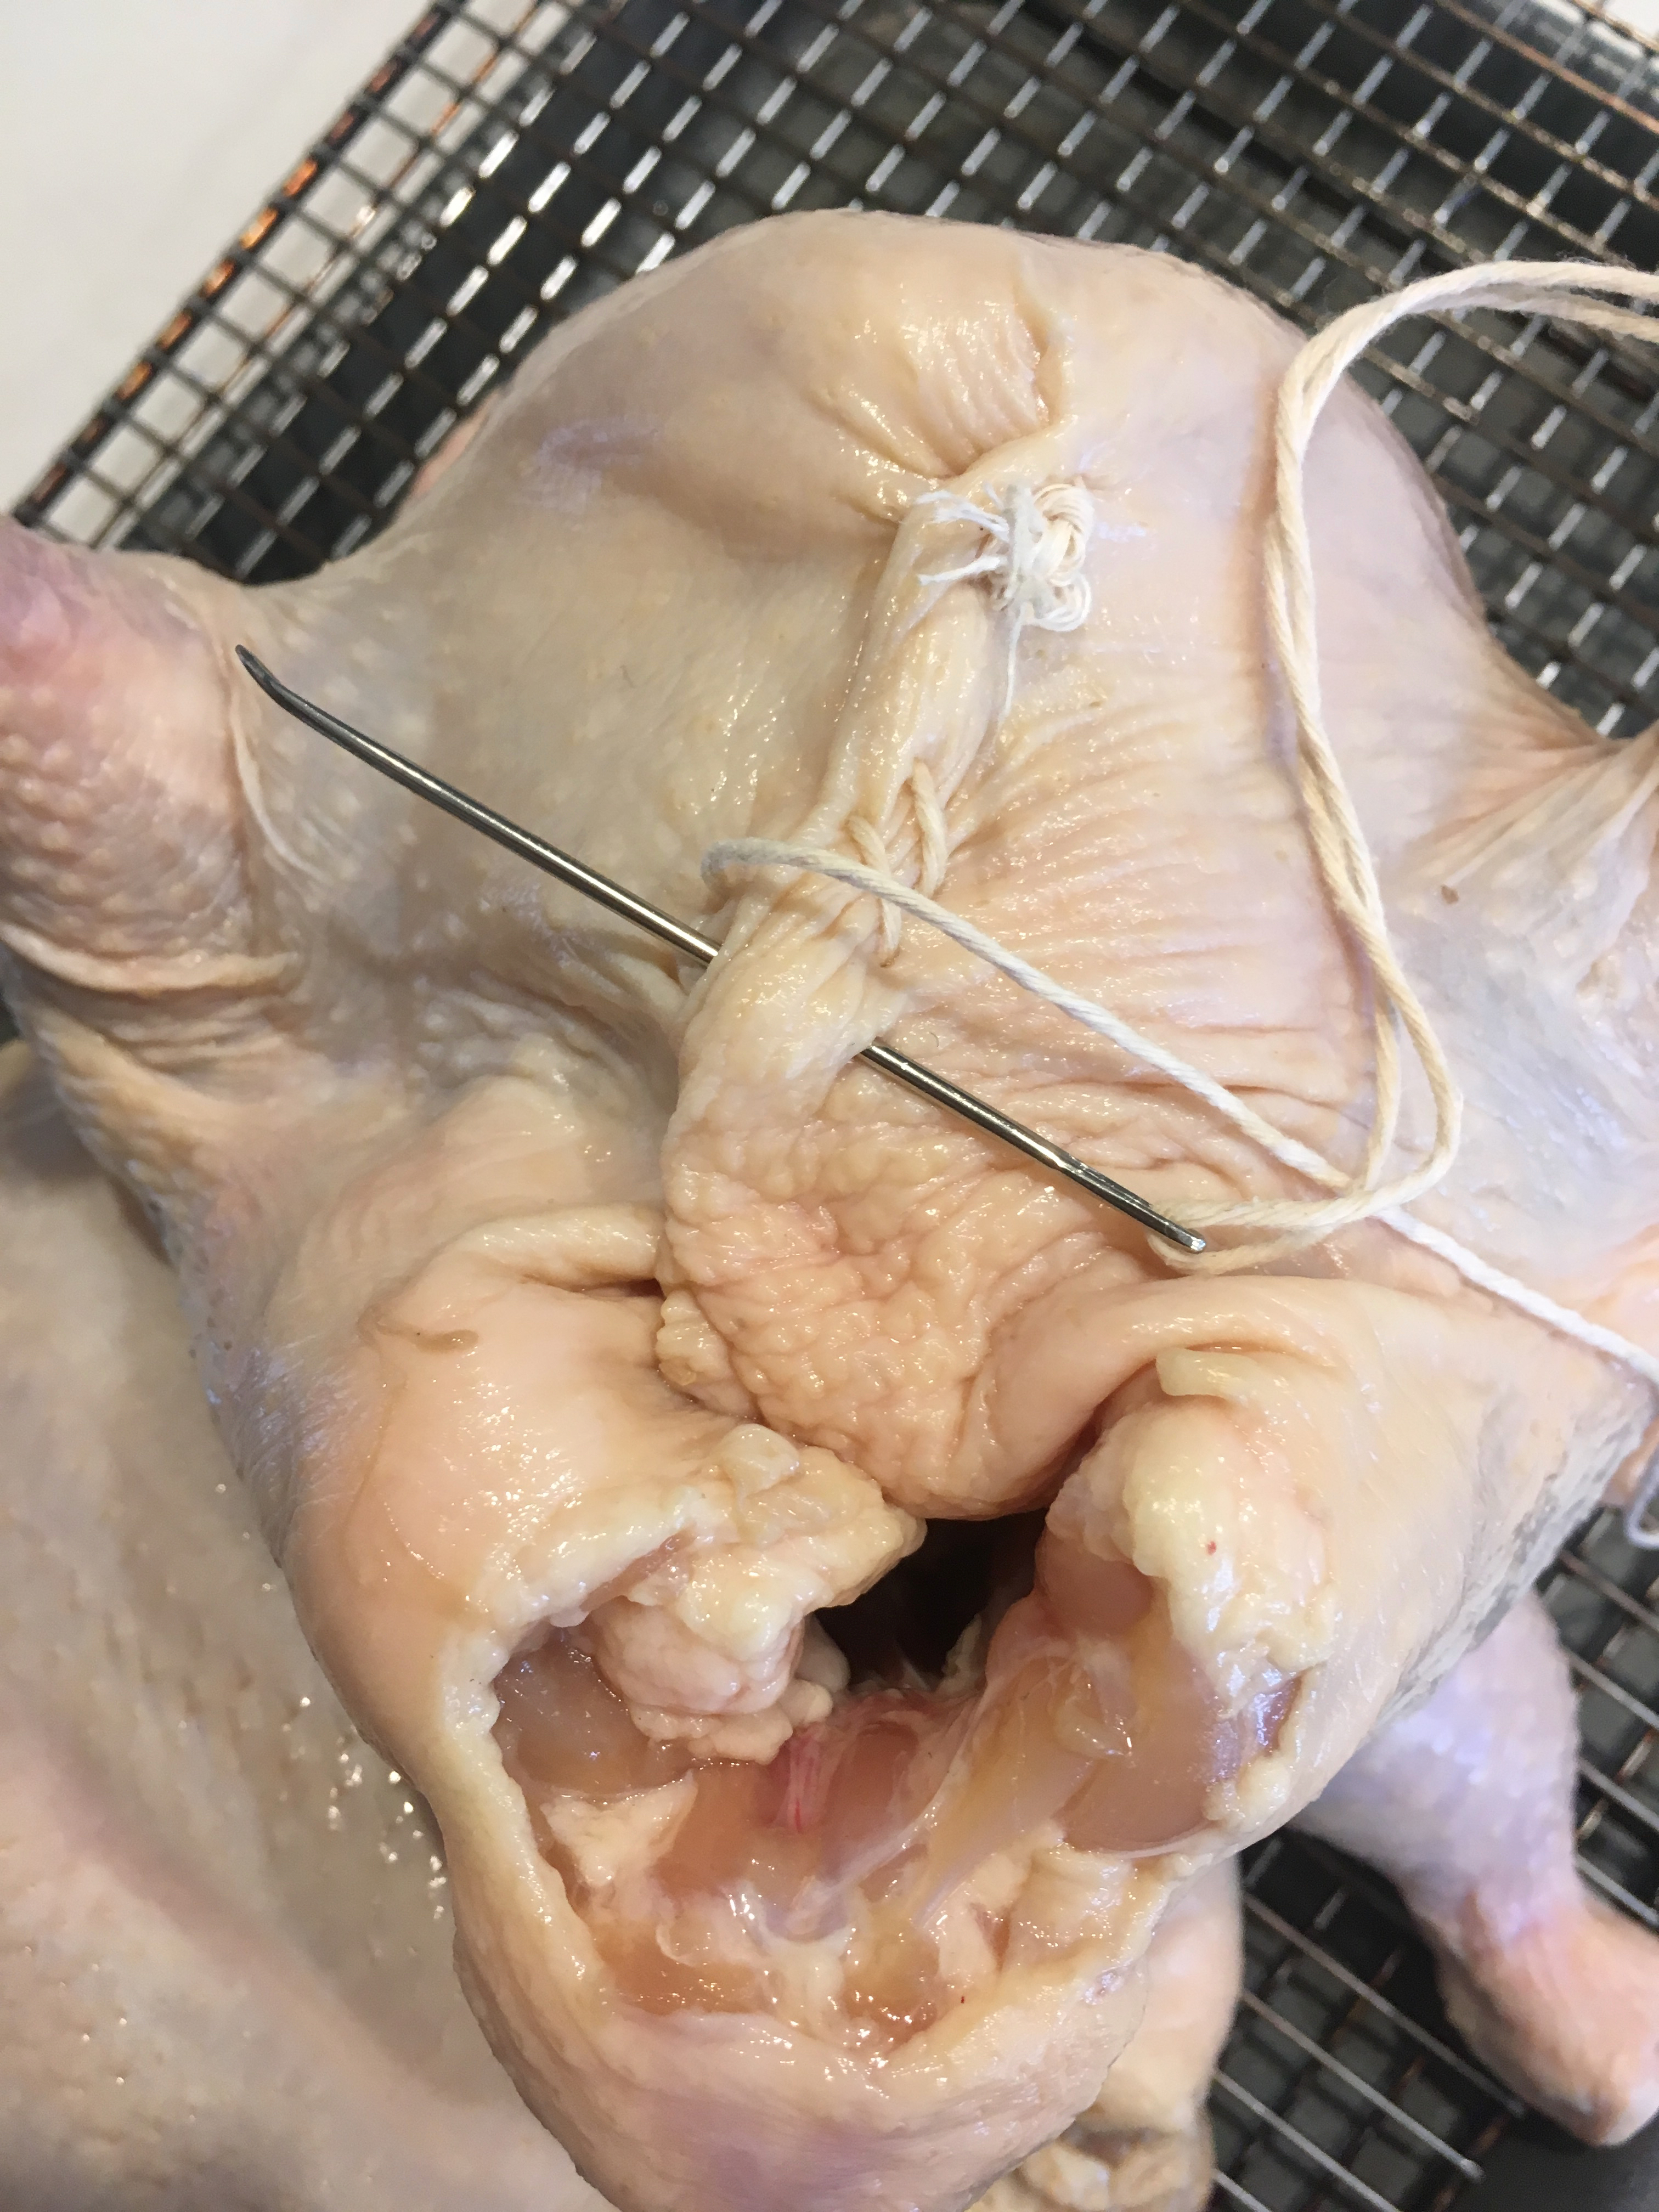
\includegraphics[width=0.25\textwidth]{\imageDir/\fileName/IMG_3214.jpg} &
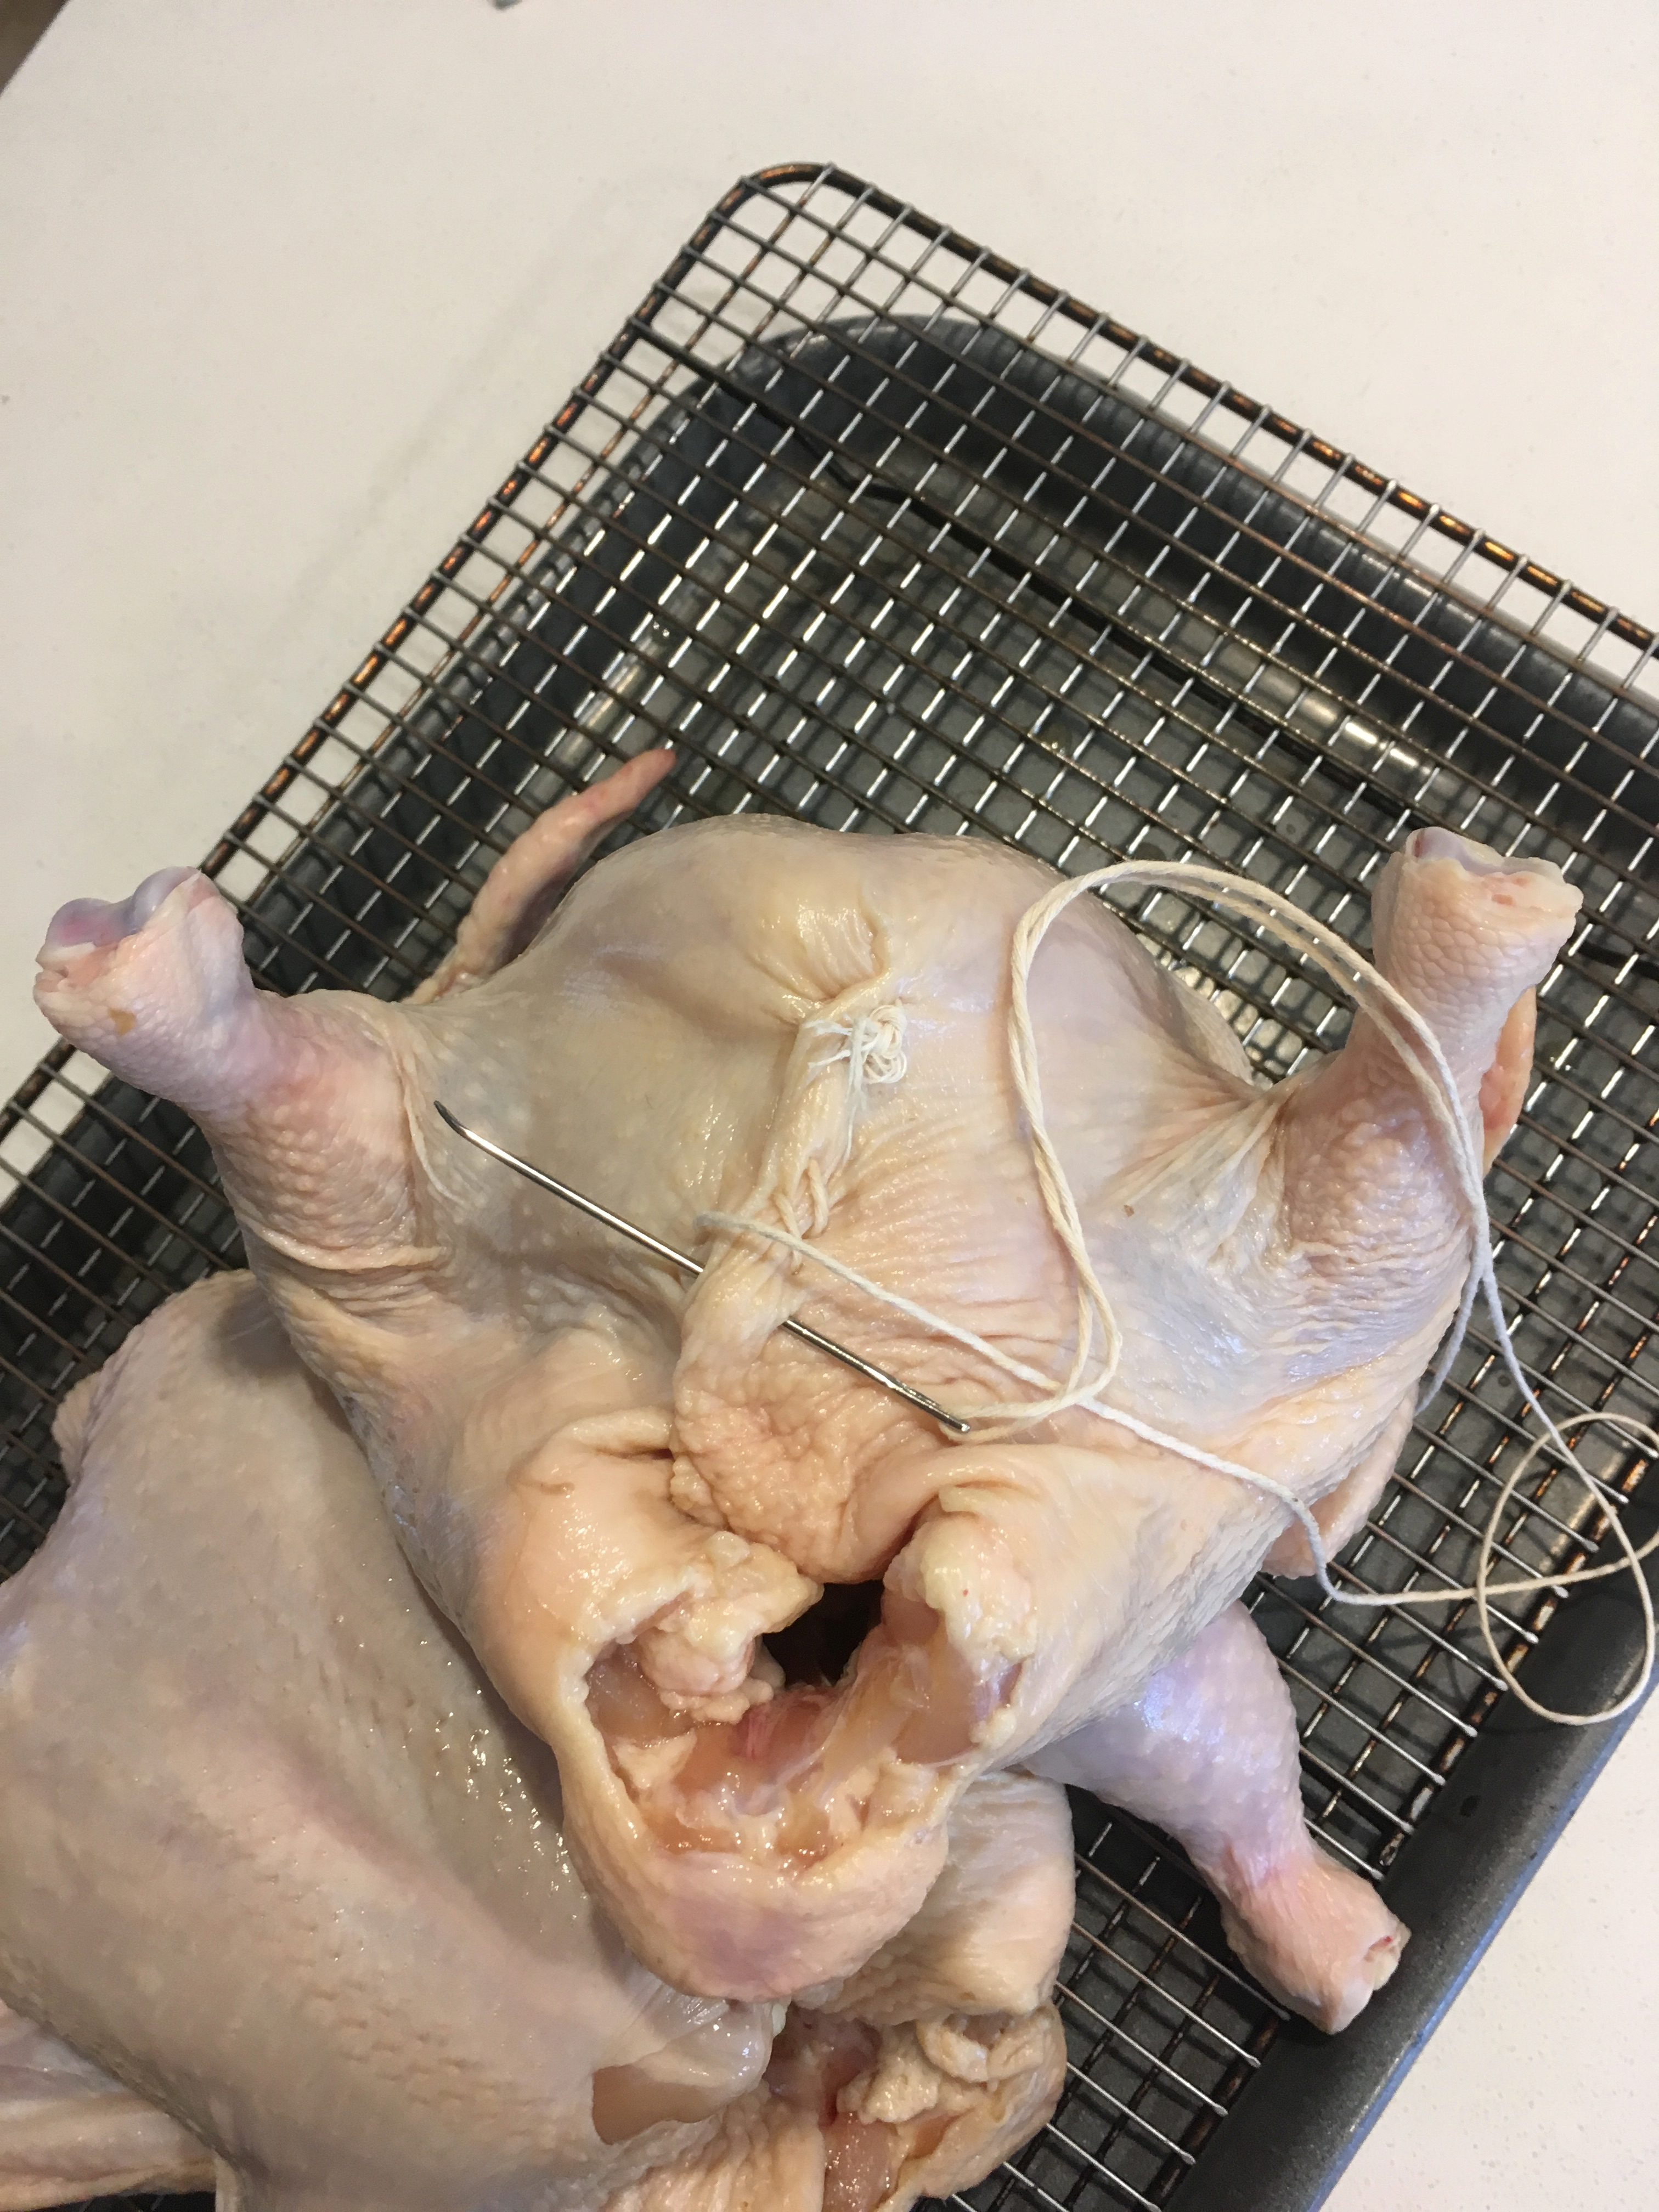
\includegraphics[width=0.25\textwidth]{\imageDir/\fileName/IMG_3216.jpg} \\
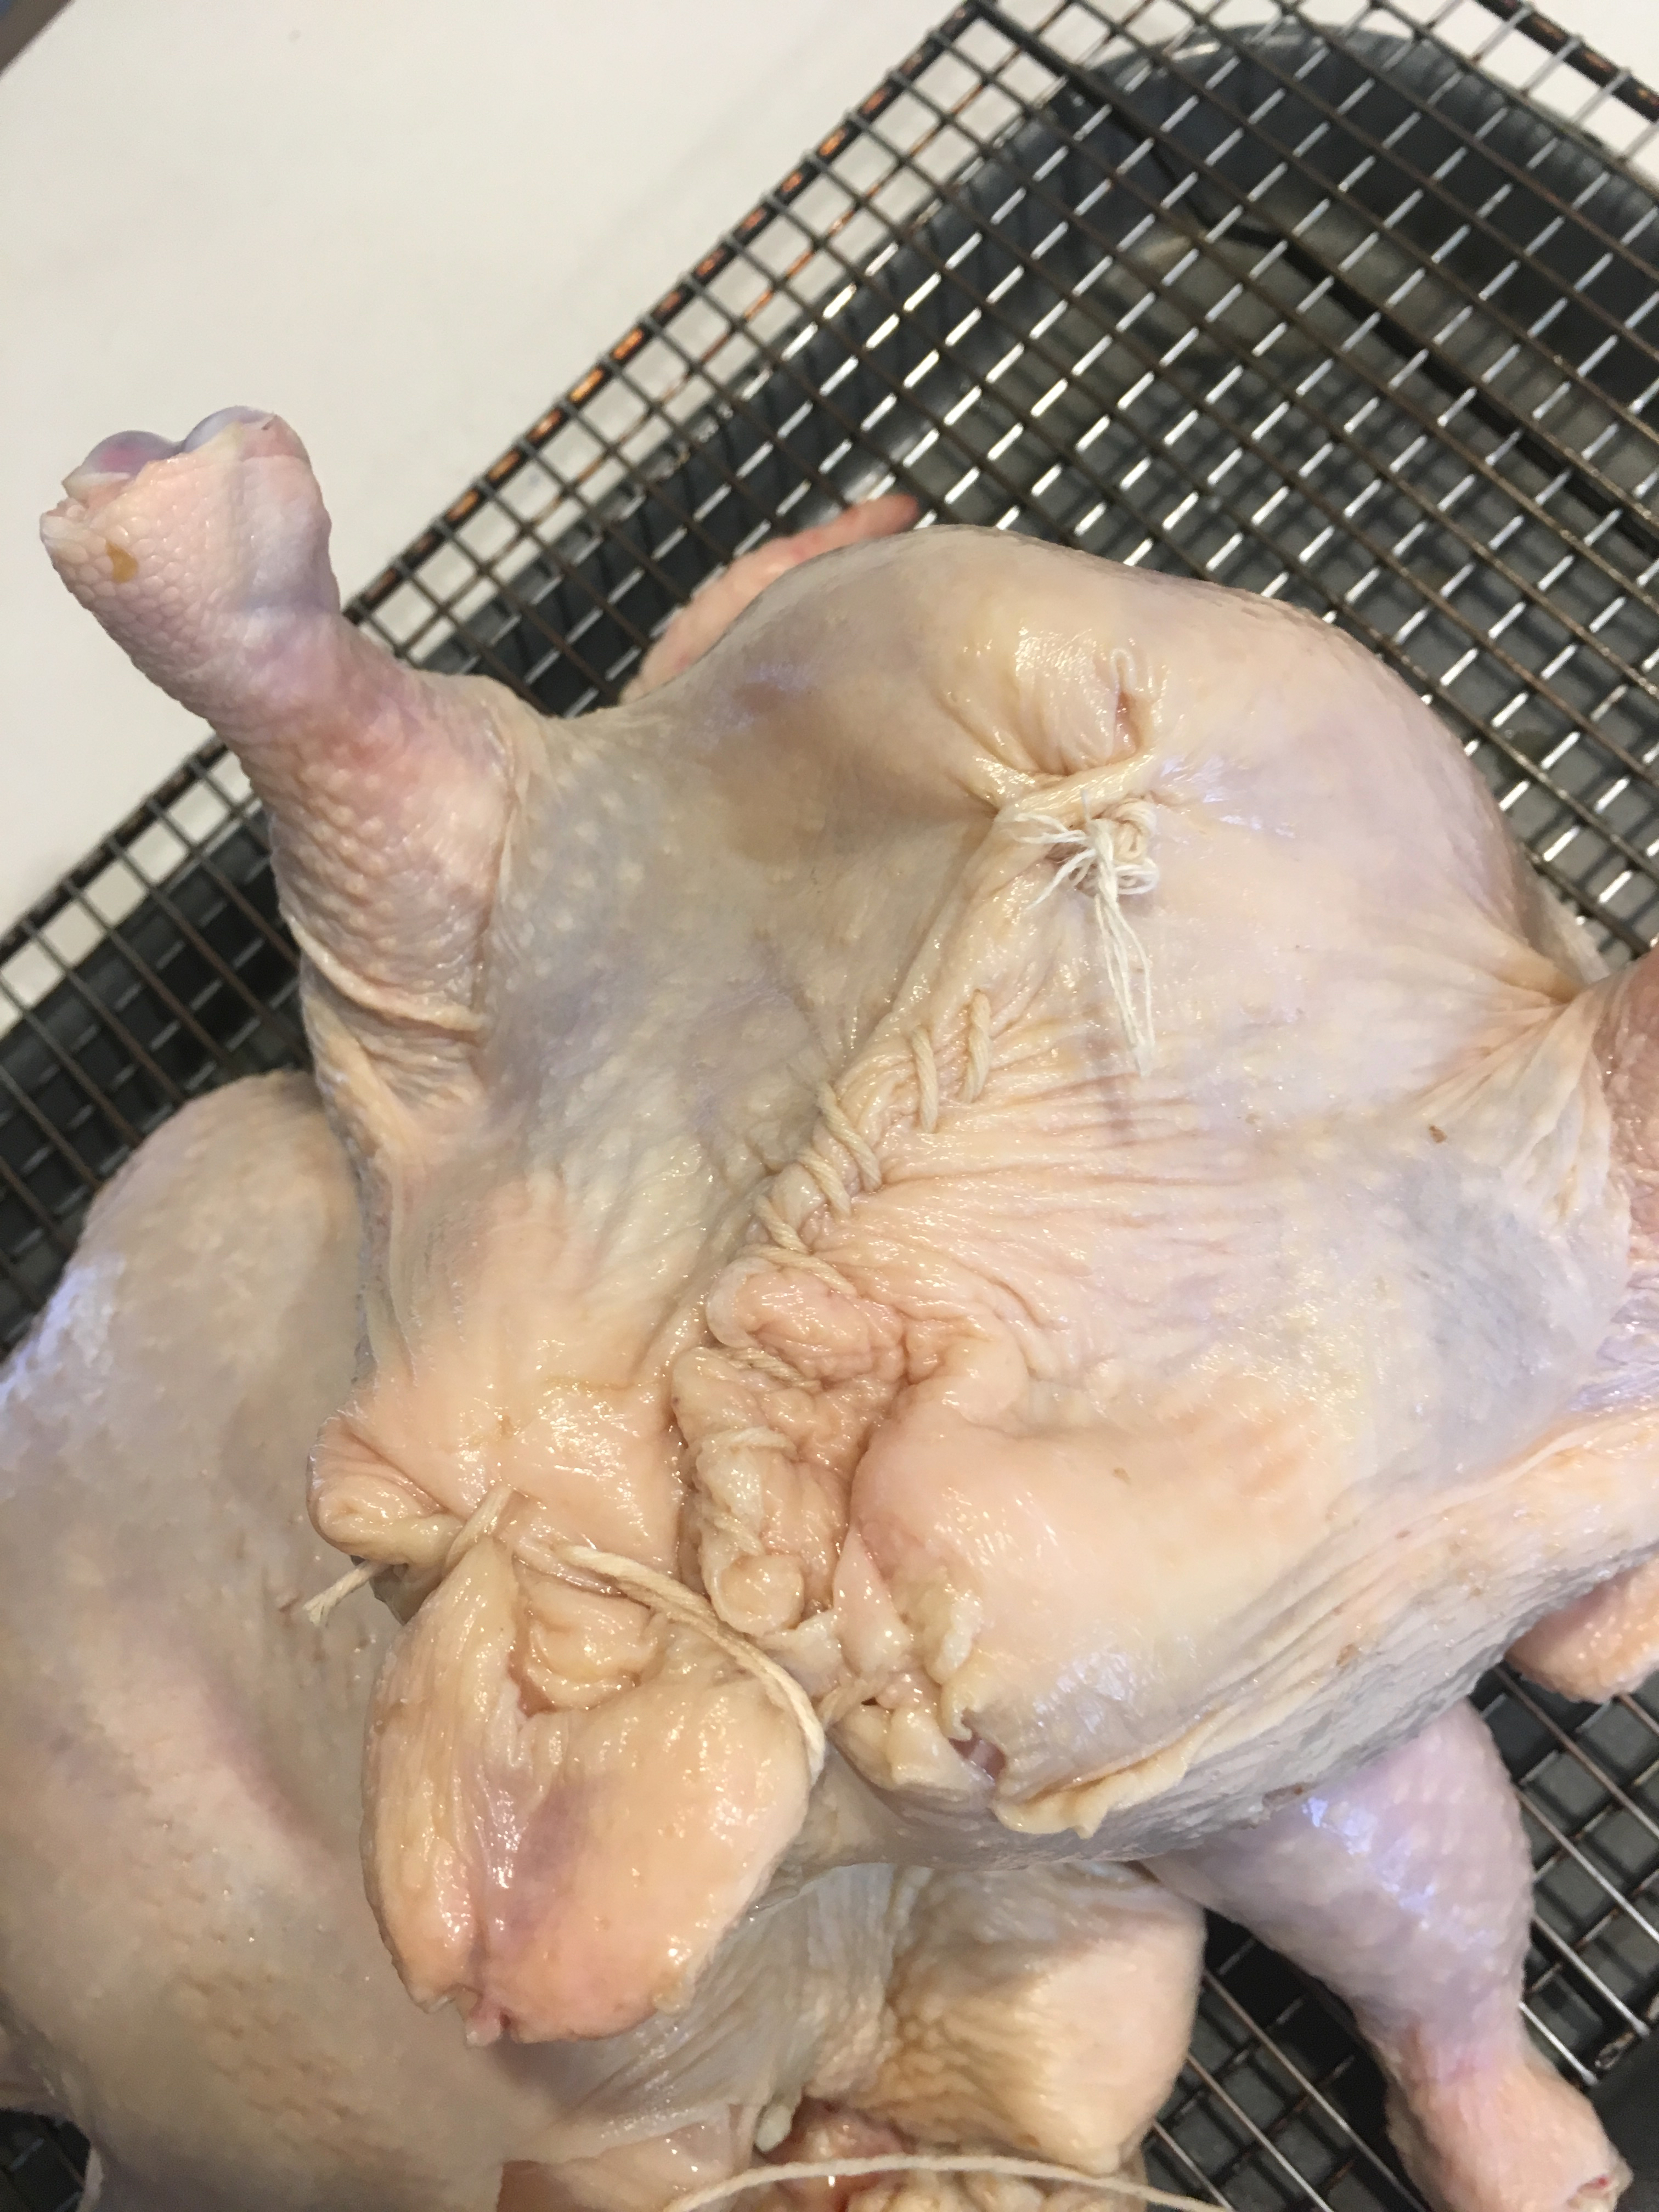
\includegraphics[width=0.25\textwidth]{\imageDir/\fileName/IMG_3217.jpg} &
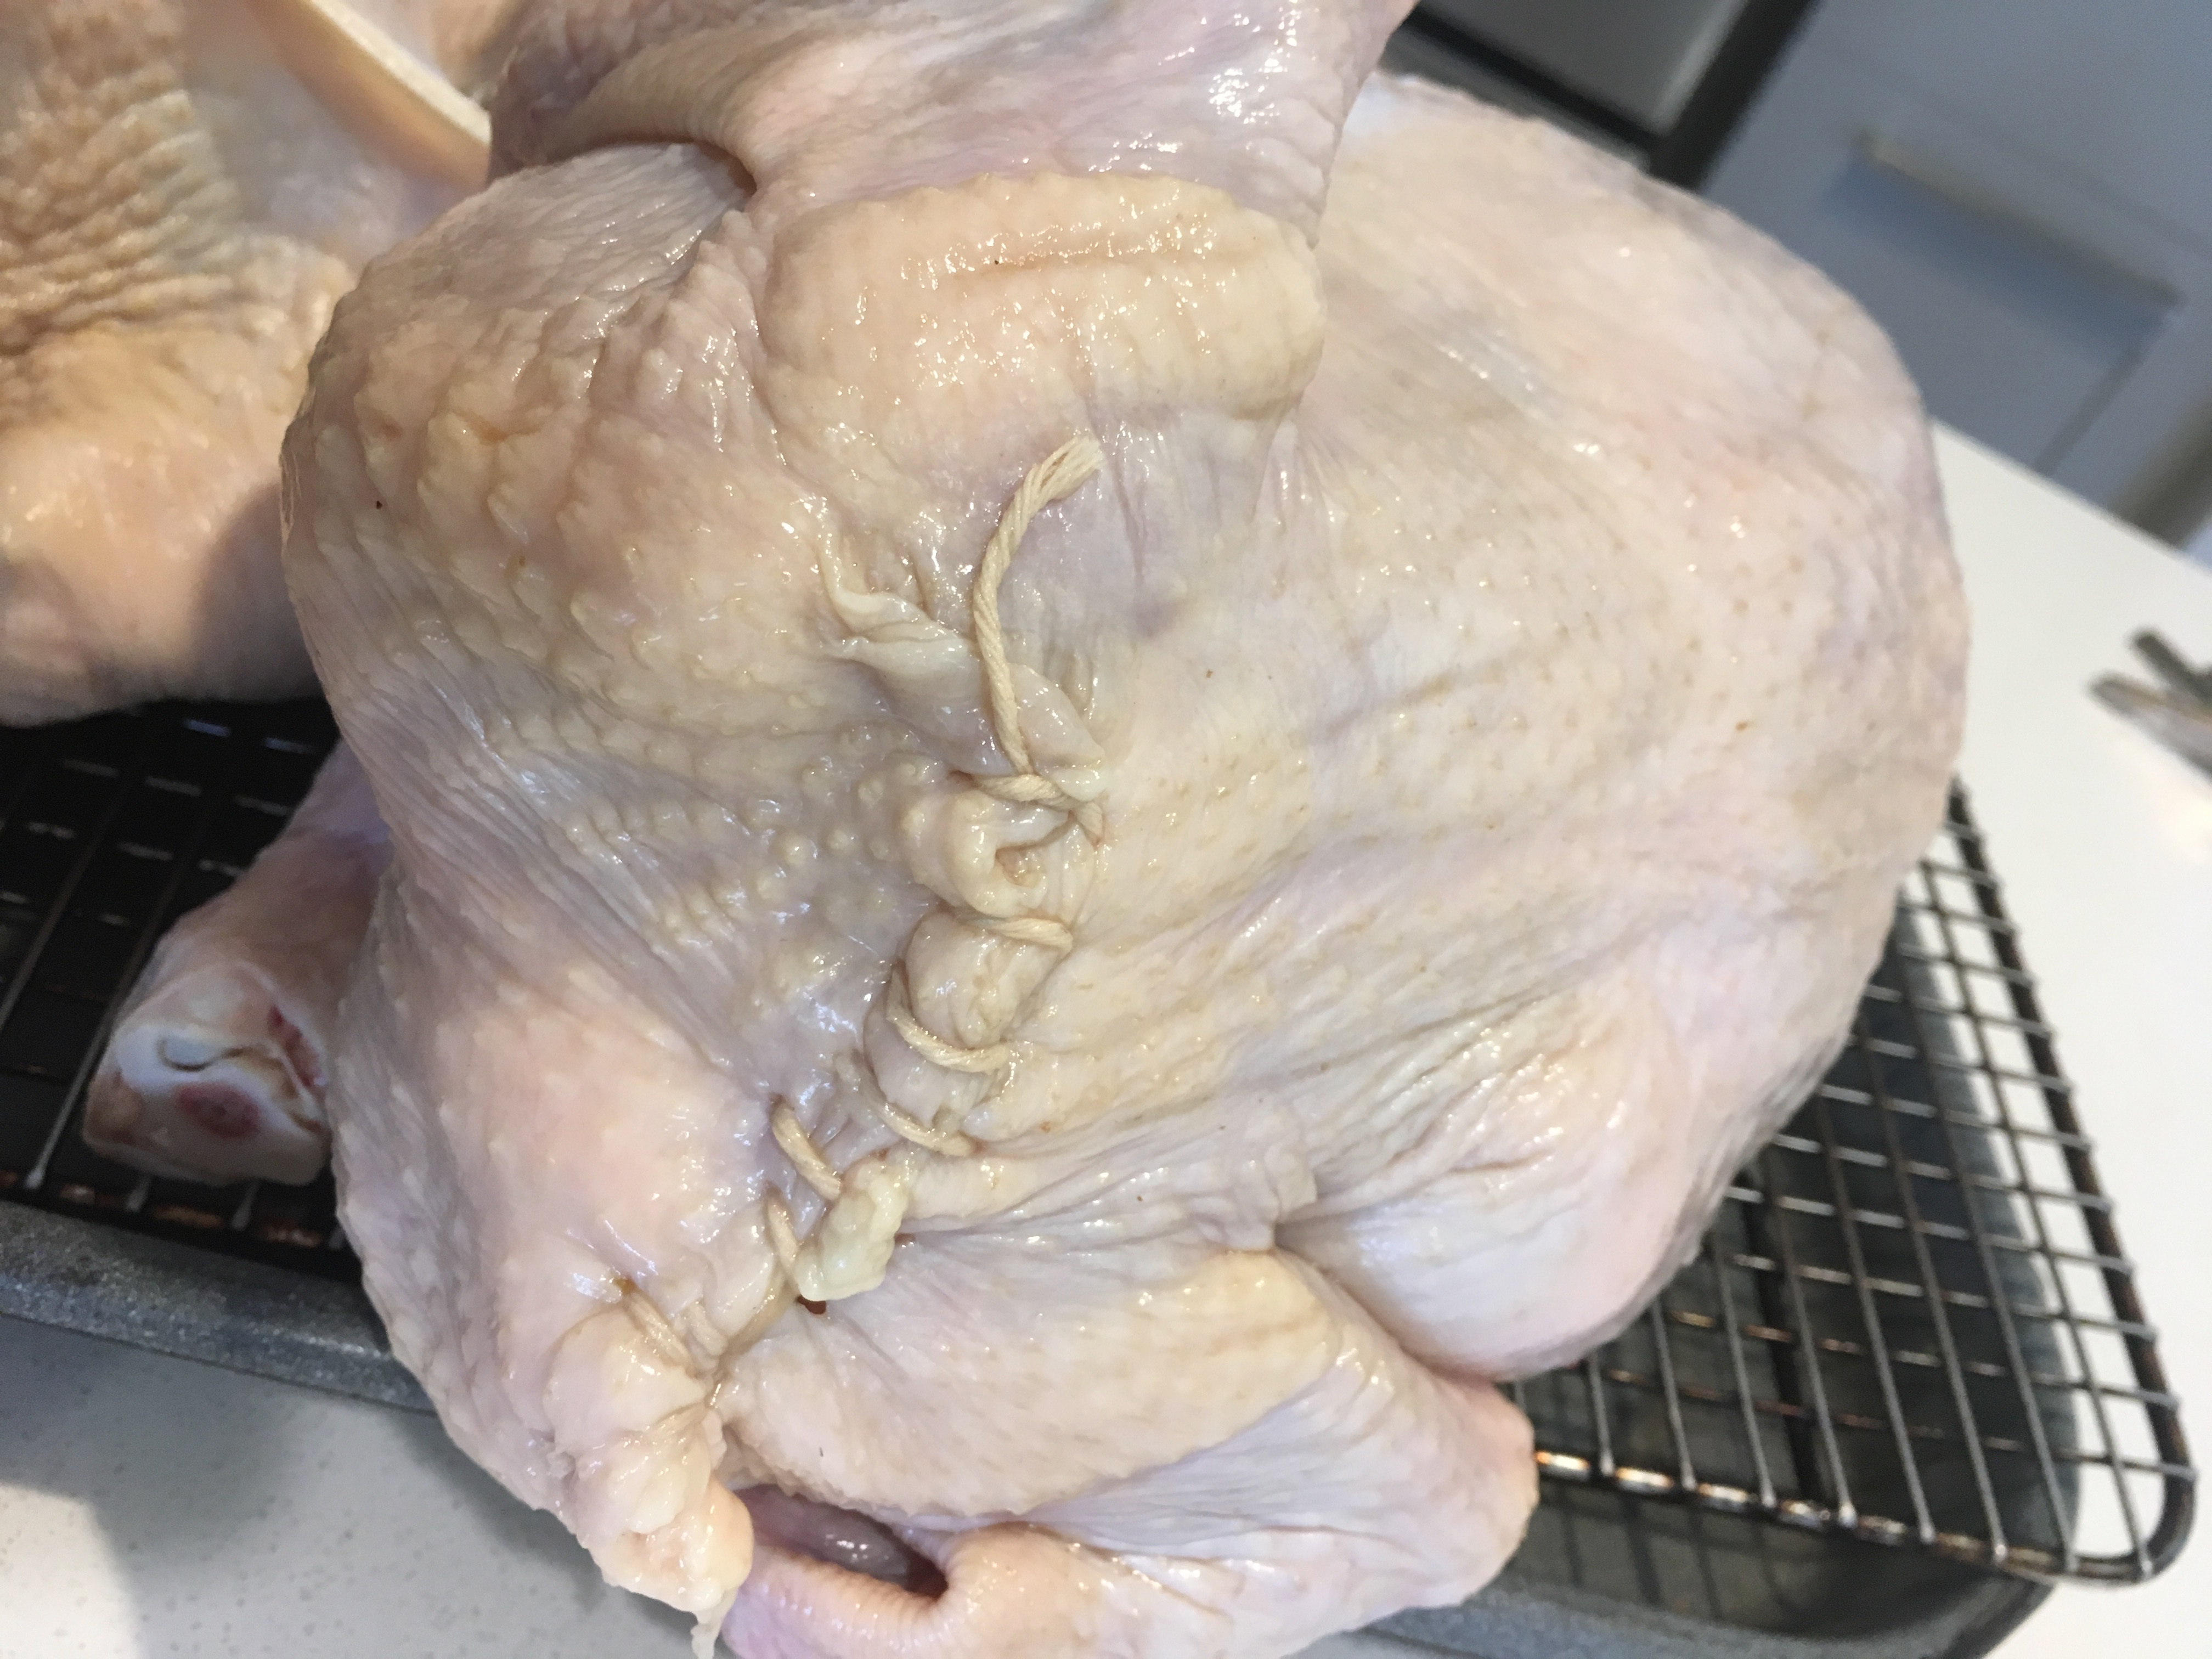
\includegraphics[width=0.25\textwidth]{\imageDir/\fileName/IMG_3218.jpg} &
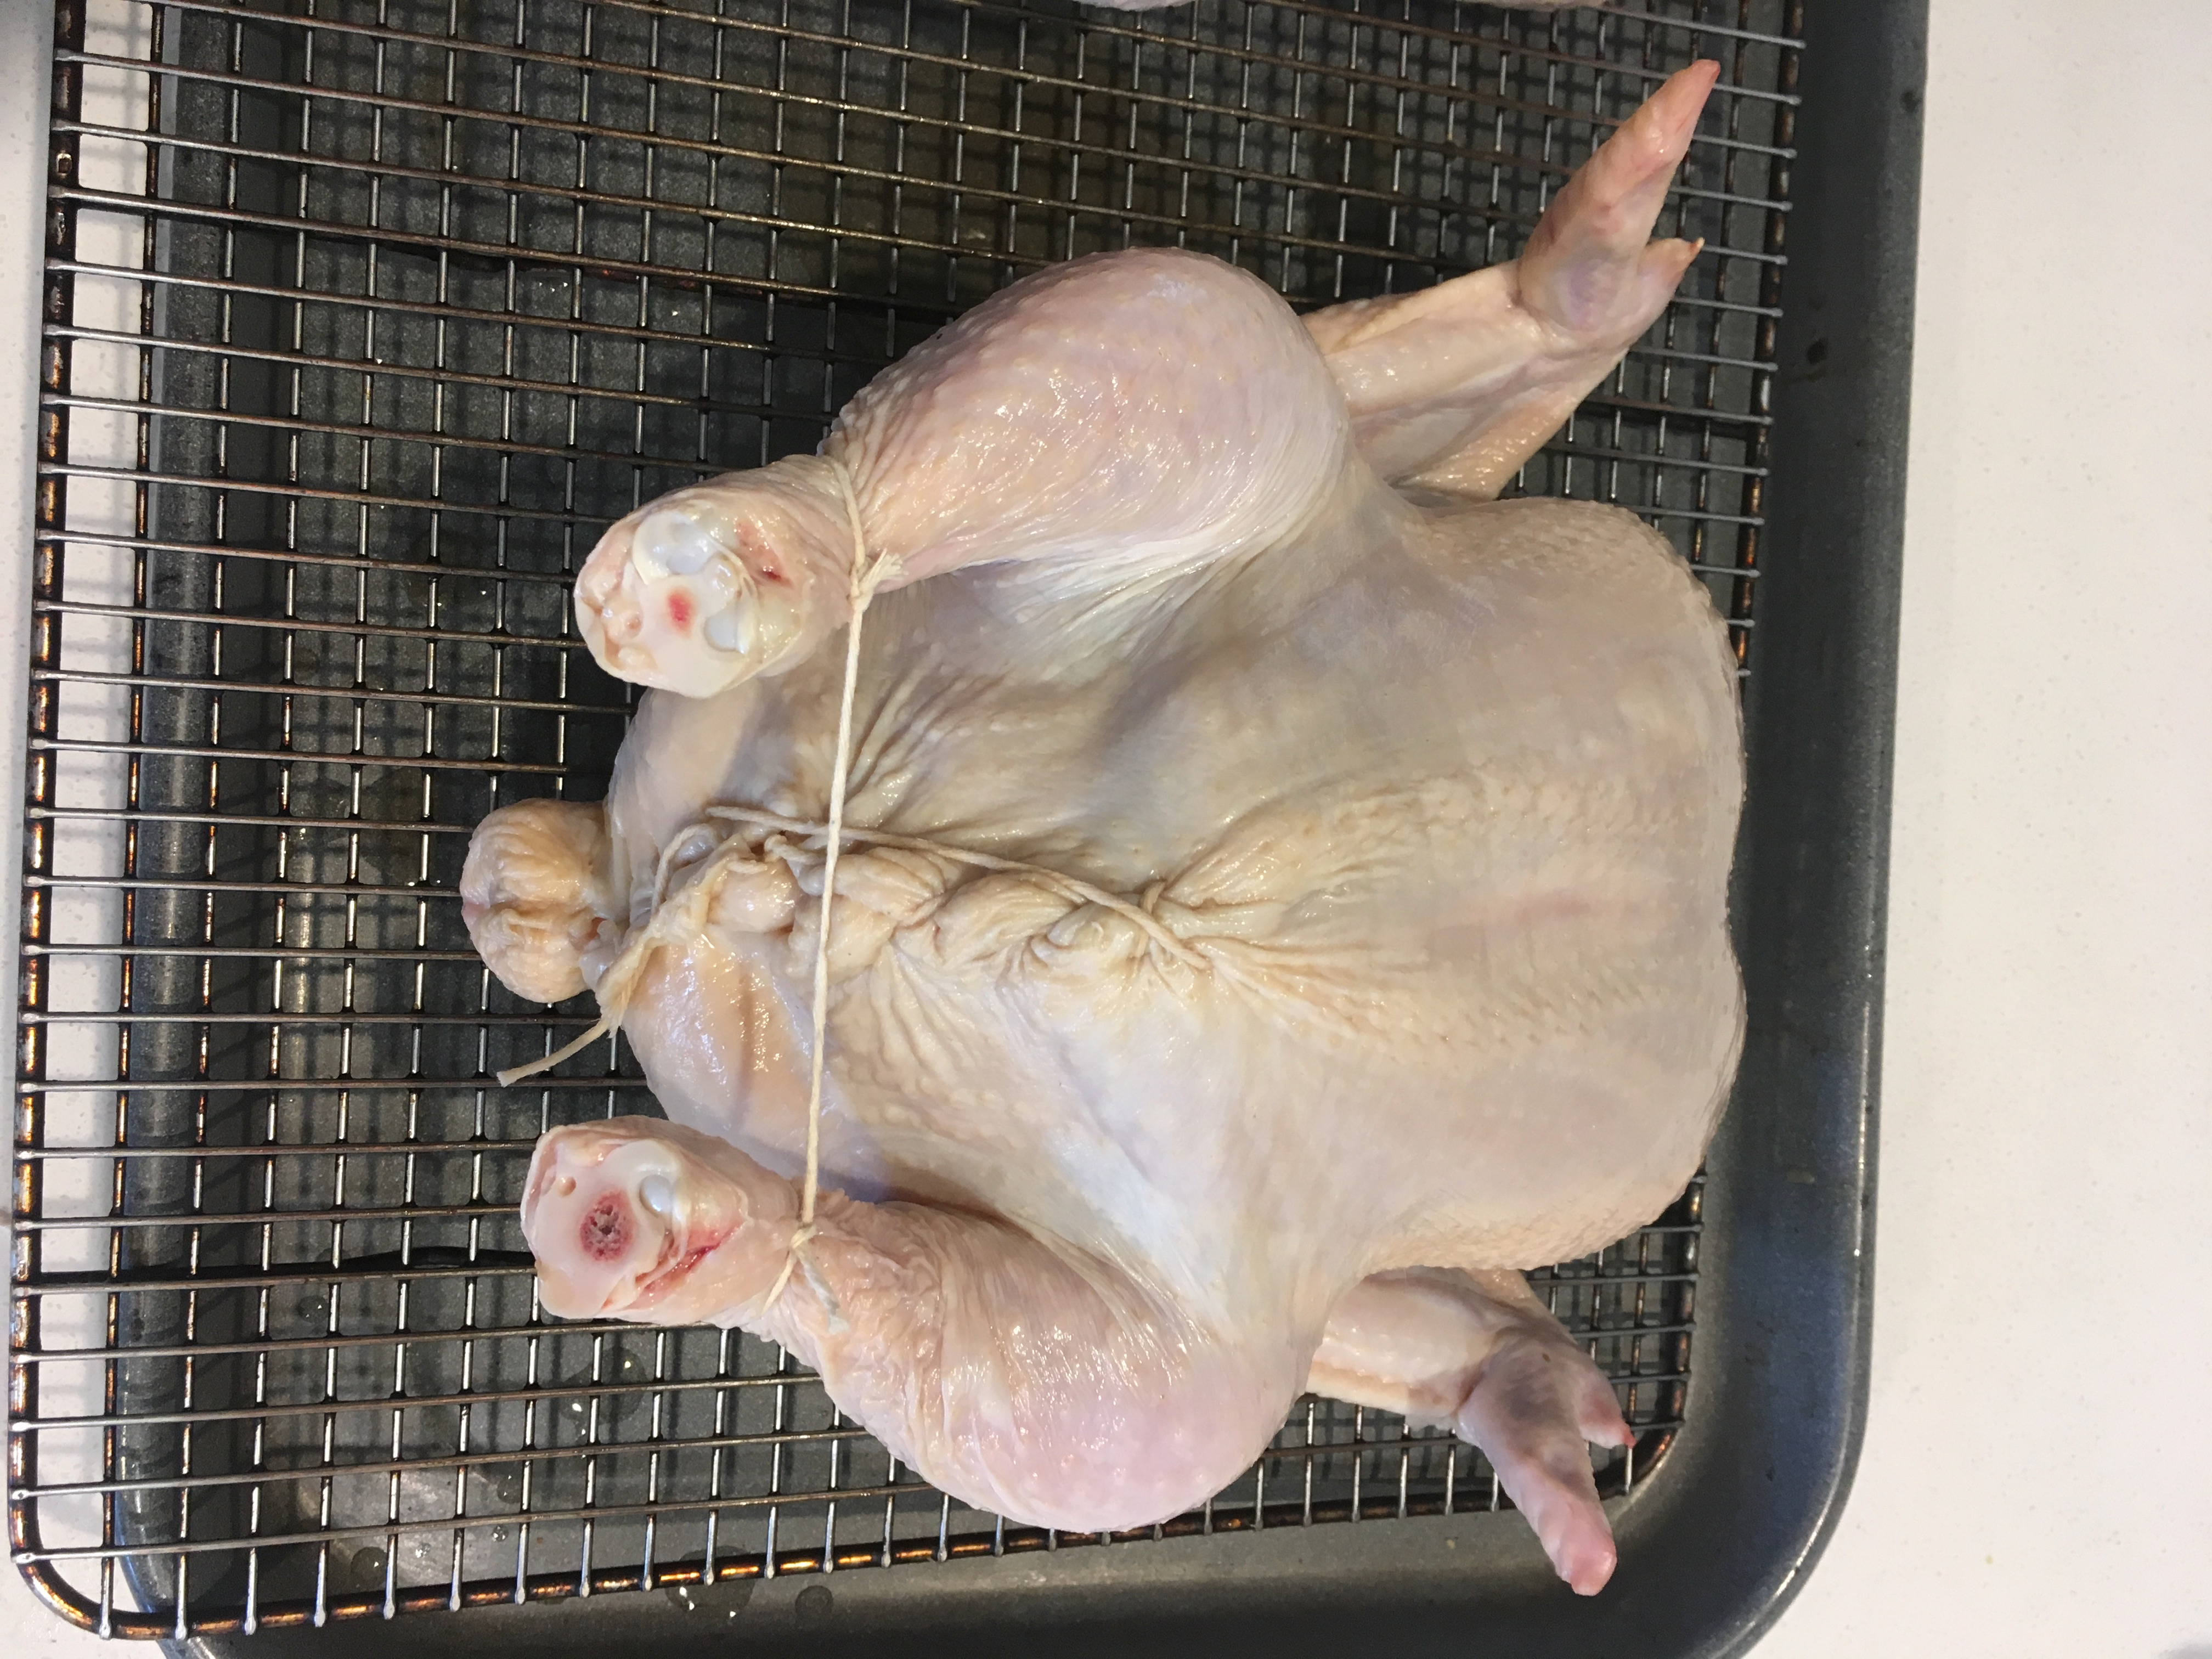
\includegraphics[width=0.25\textwidth]{\imageDir/\fileName/IMG_3219.jpg} \\
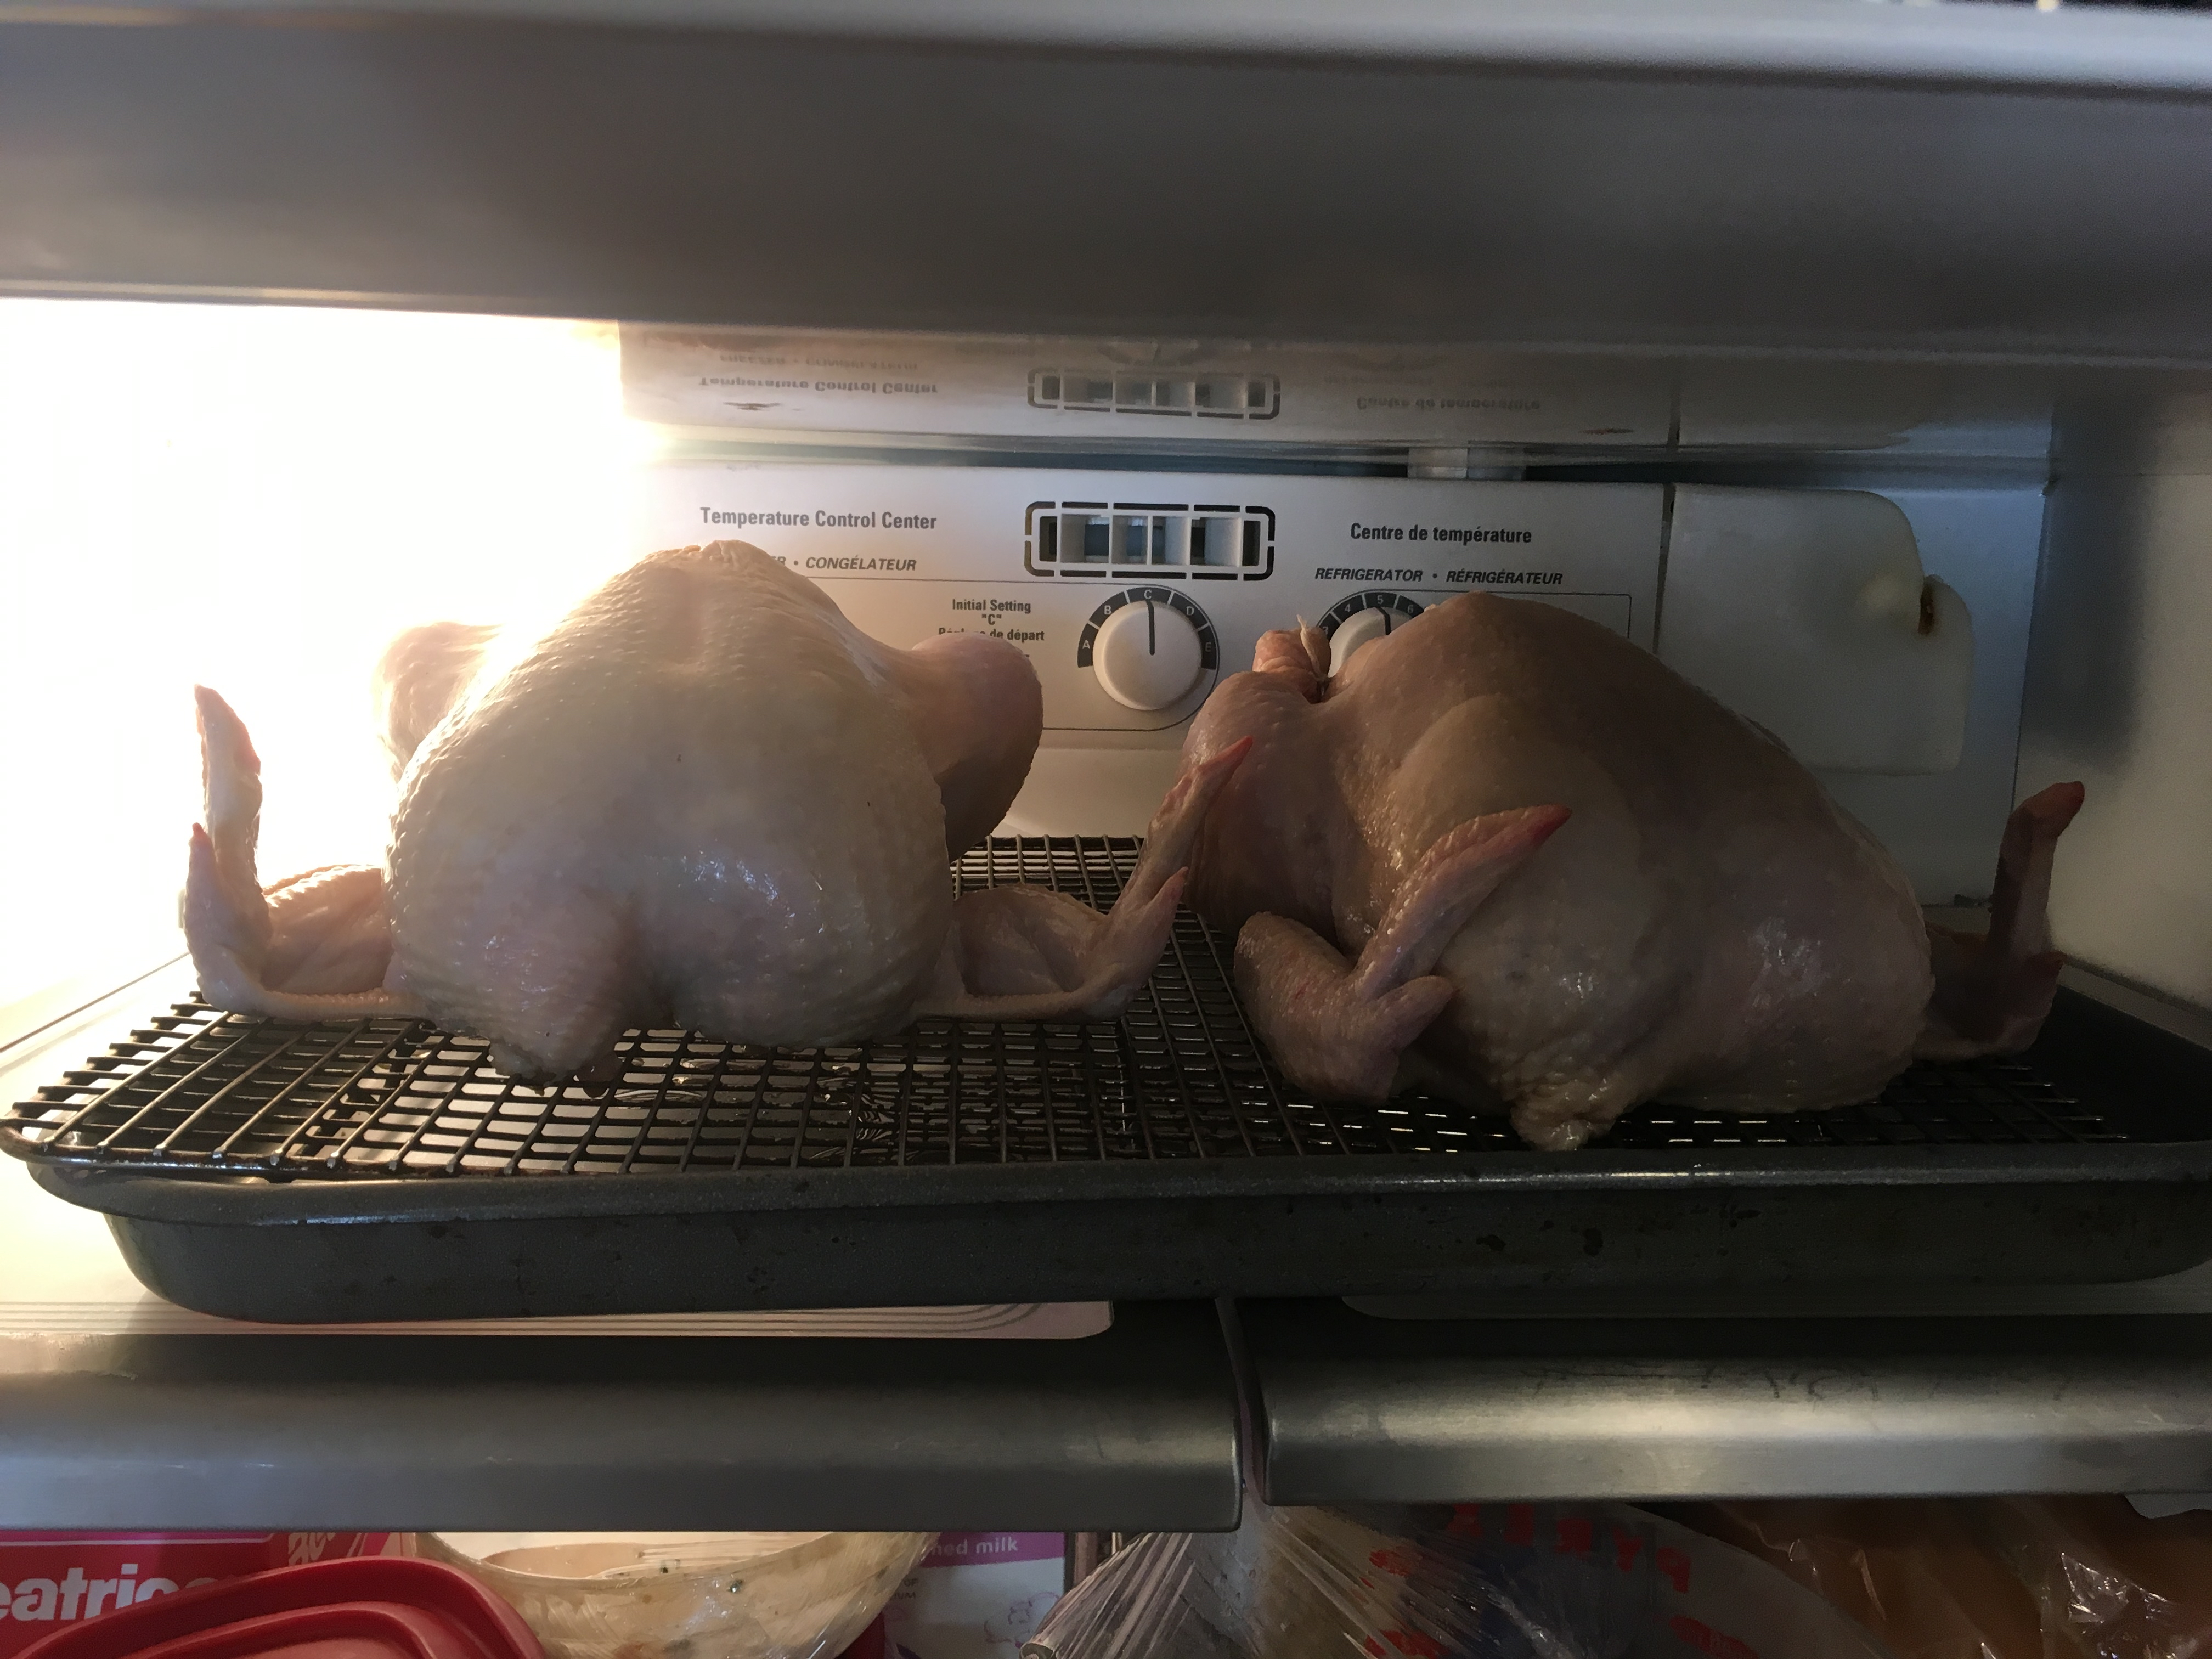
\includegraphics[width=0.25\textwidth]{\imageDir/\fileName/IMG_3220.jpg} &
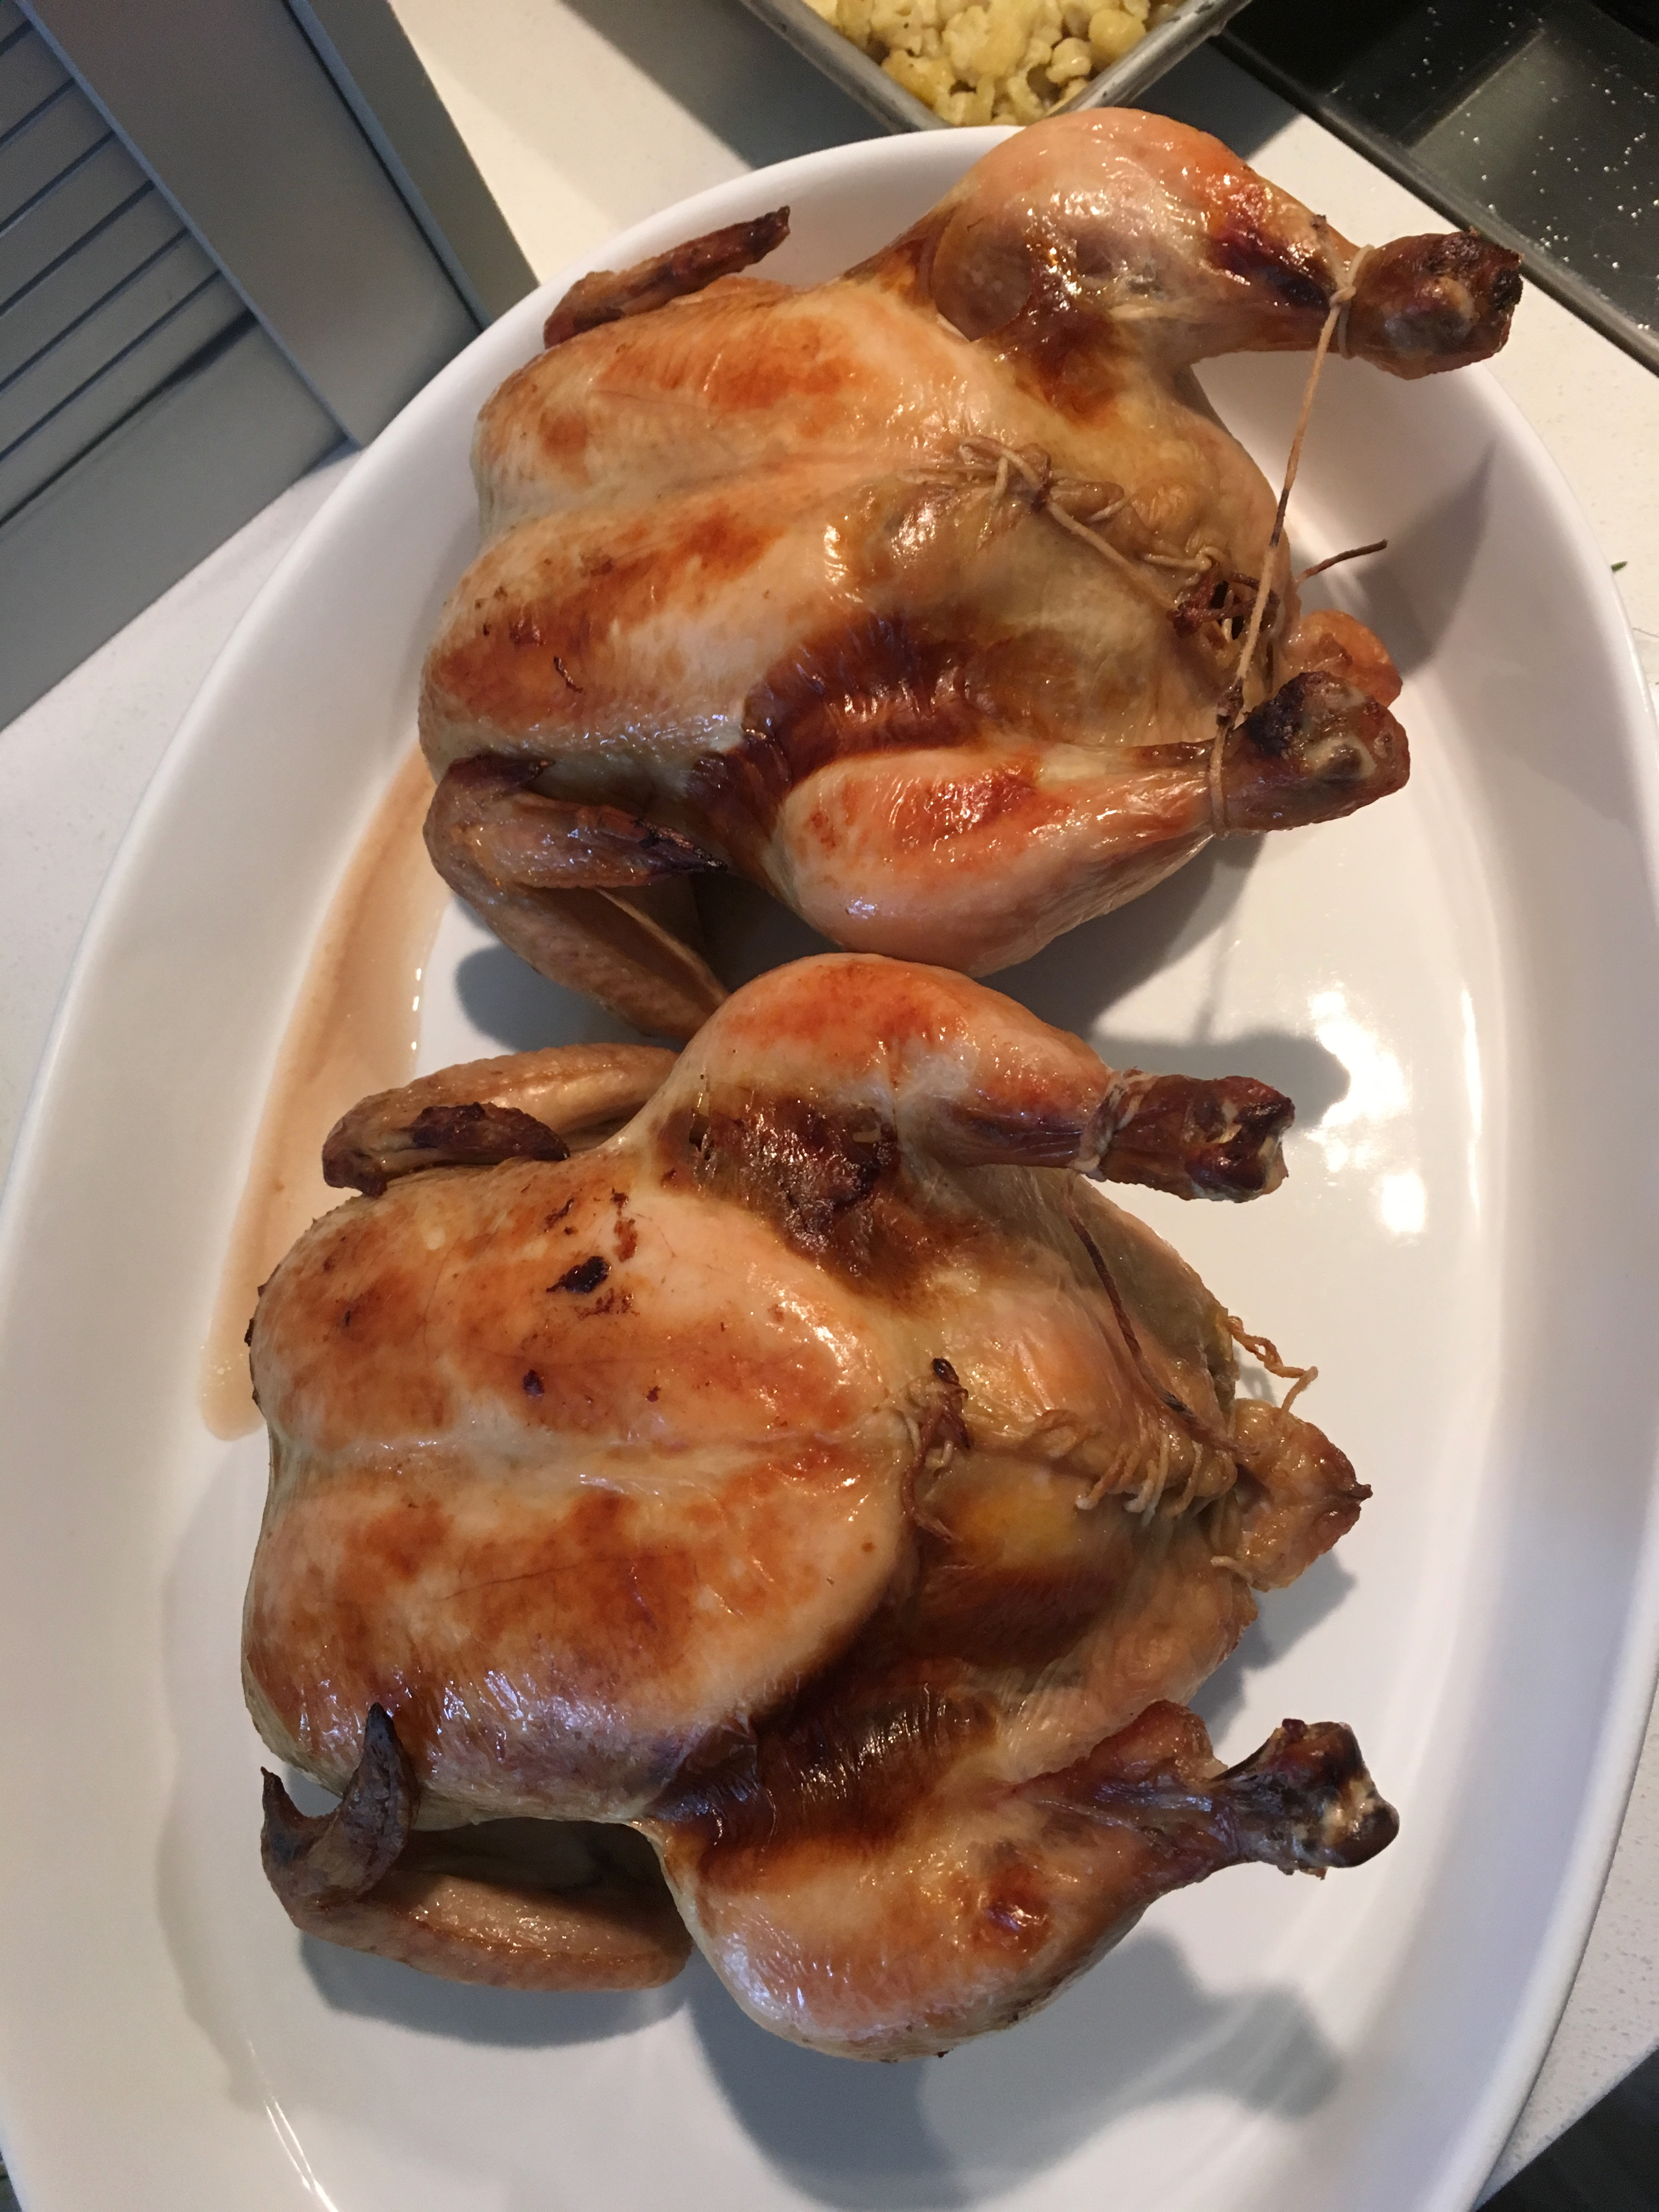
\includegraphics[width=0.25\textwidth]{\imageDir/\fileName/IMG_3228.jpg} \\
\end{tabular}
\end{table}


\end{document}
